
\subsection{Sơ đồ Use Case chi tiết xác thực}
\begin{figure}[H]
    \centering
    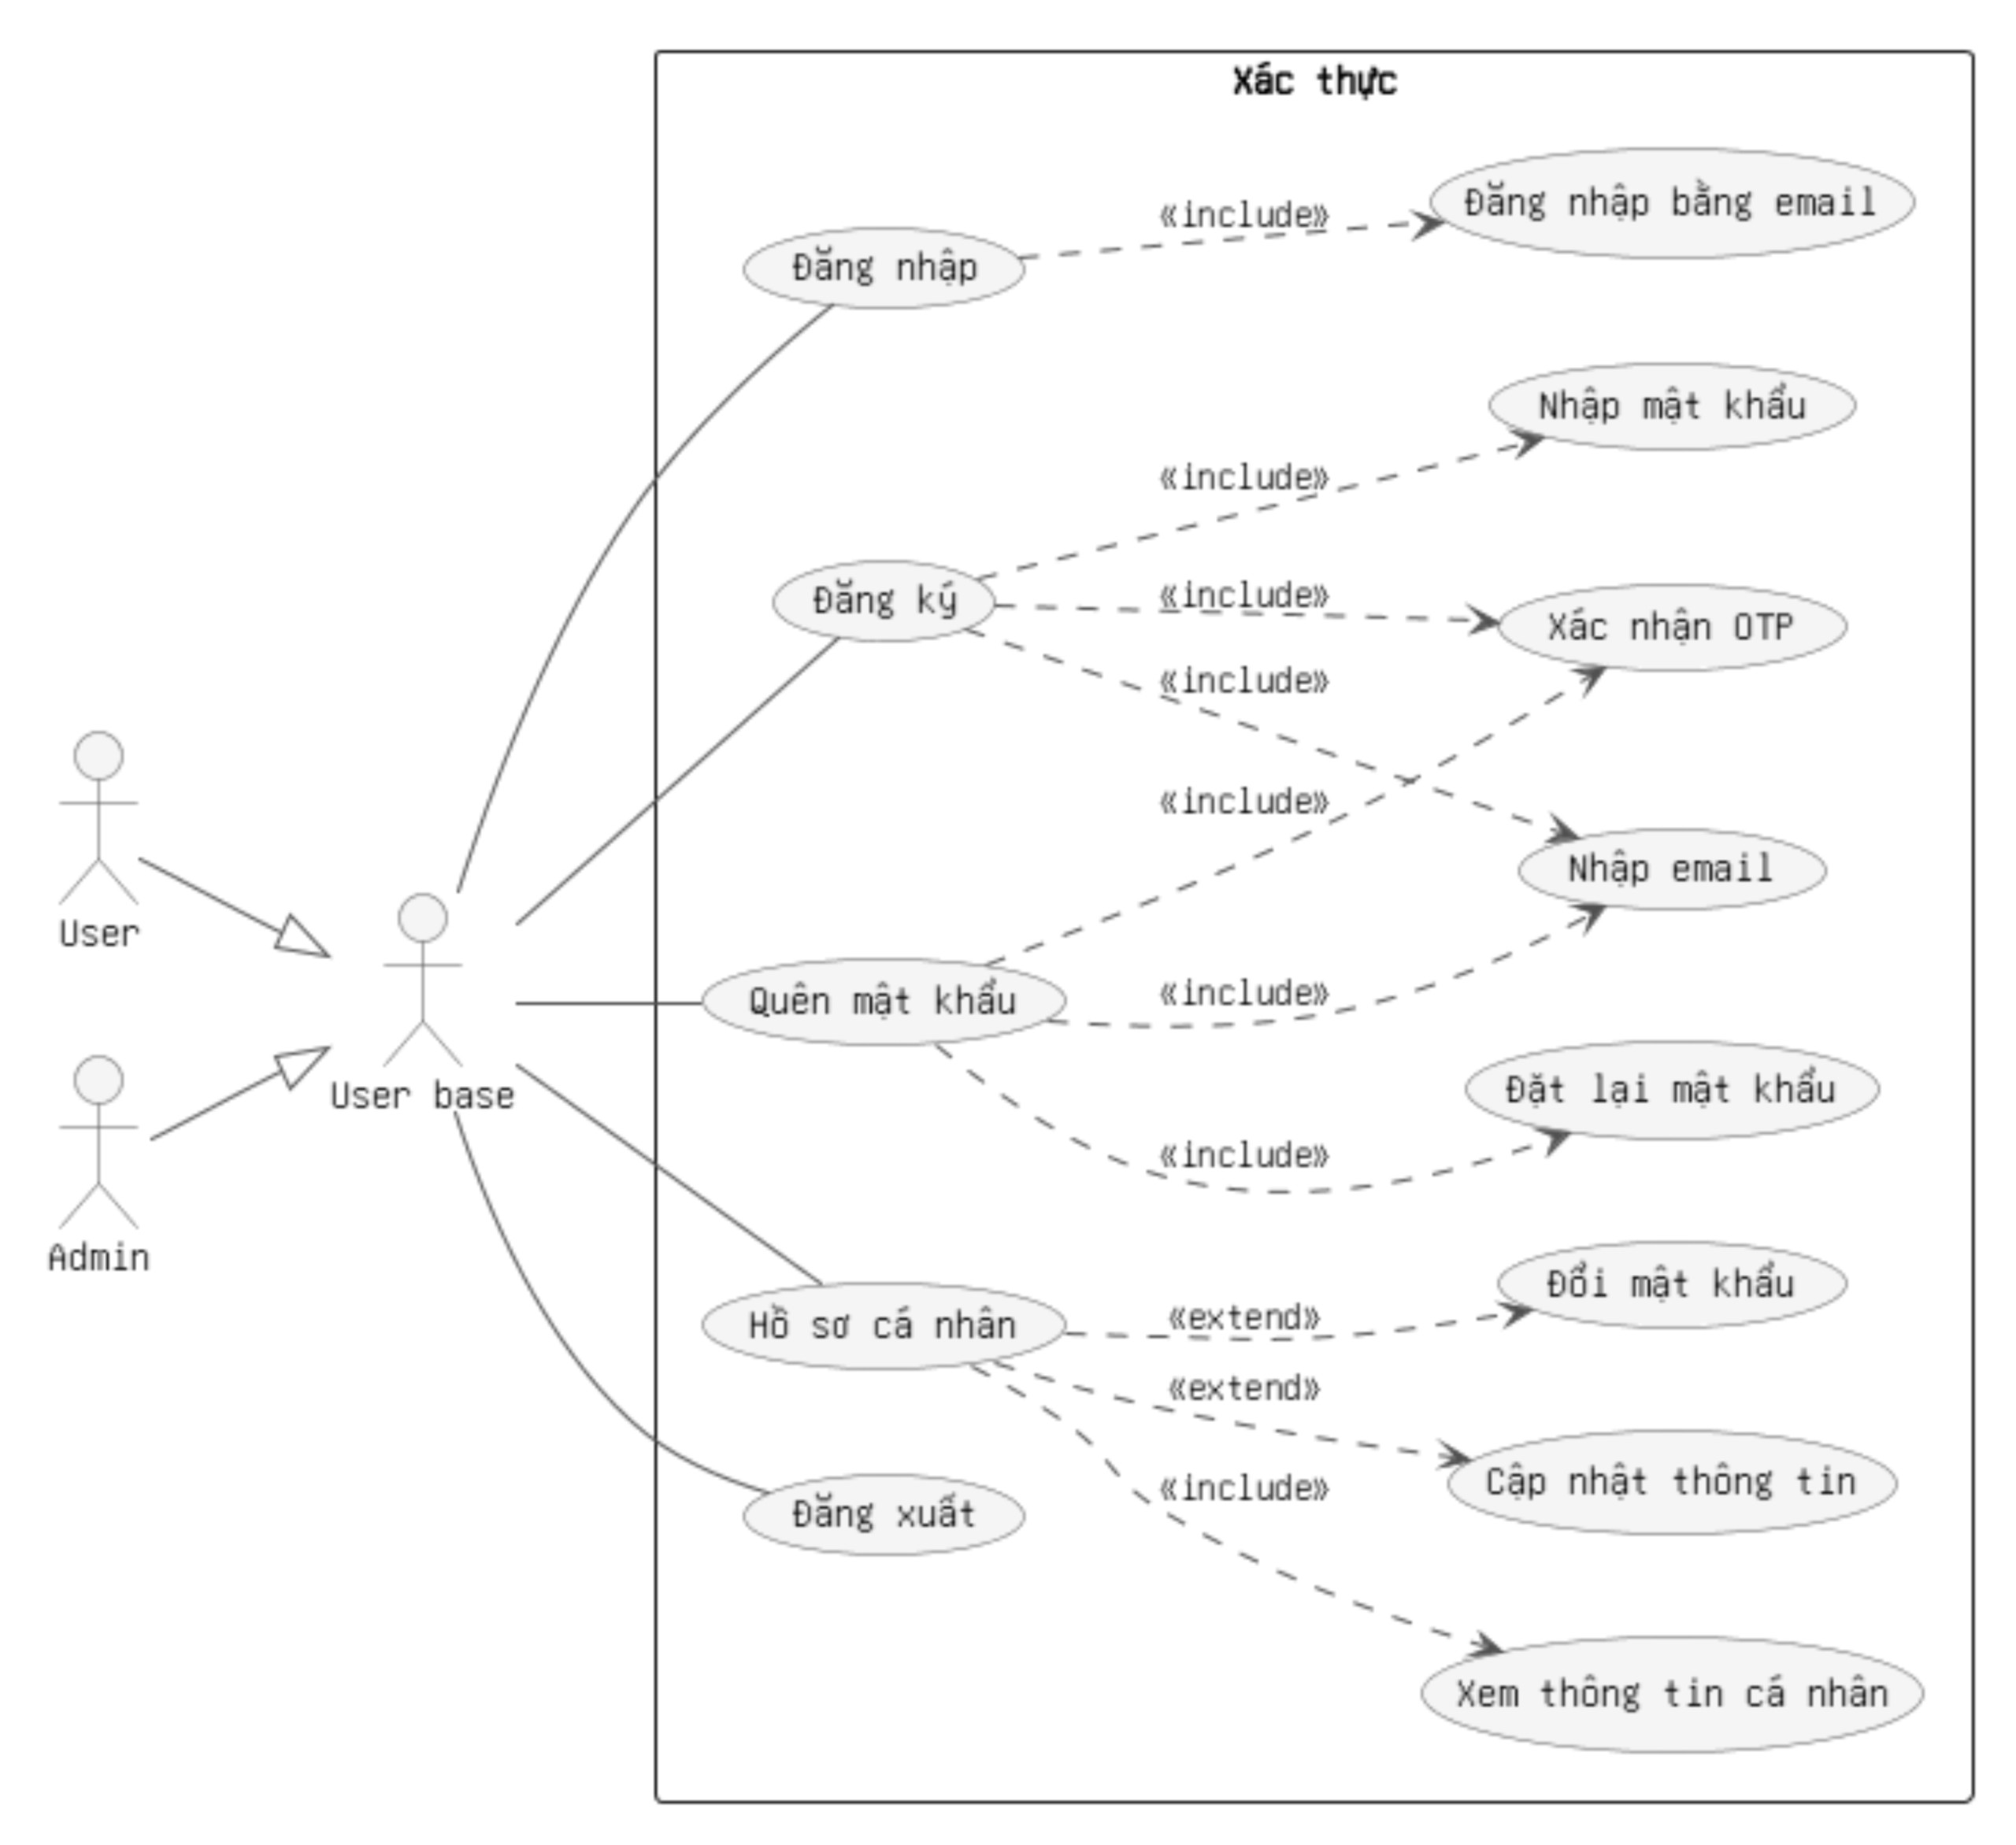
\includegraphics[width=1.0\textwidth]{figures/uc_xac_thuc.jpg}
    \caption{Sơ đồ Use Case  chi tiết xác thực}
    \label{fig:usecase_xac_thuc}
\end{figure}



\subsection*{UC01 -- Đăng nhập}
\begin{table}[H]
    \captionsetup{justification=raggedright, singlelinecheck=false}
    \caption{Đặc tả UC01 -- Đăng nhập}
\centering
\begin{tabular}{|p{3.5cm}|p{10cm}|}
\hline
\textbf{Tên use case} & Đăng nhập \\
\hline
\textbf{Actor} & User base (User, Admin) \\
\hline
\textbf{Mô tả} & Người dùng xác thực tài khoản để truy cập hệ thống \\
\hline
\textbf{Tiền điều kiện} & Người dùng đã có tài khoản \\
\hline
\textbf{Hậu điều kiện} & Người dùng được cấp token và vào Dashboard \\
\hline
\textbf{Luồng chính} &
  1. Người dùng nhập email và mật khẩu \newline
  2. Hệ thống xác thực qua Firebase Auth \newline
  3. Hệ thống cấp token và chuyển vào Dashboard \\
\hline
\textbf{Luồng thay thế} &
  2a. Sai thông tin: thông báo lỗi, quay lại bước 1 \newline
  2b. Quên mật khẩu: chuyển sang UC03 \\
\hline
\textbf{Include} & Đăng nhập bằng email, Nhập mật khẩu \\
\hline
\end{tabular}

\end{table}

\subsection*{UC02 -- Đăng ký}
\begin{table}[H]
    \captionsetup{justification=raggedright, singlelinecheck=false}
    \caption{Đặc tả UC02 -- Đăng ký}
\centering
\begin{tabular}{|p{3.5cm}|p{10cm}|}
\hline
\textbf{Tên use case} & Đăng ký \\
\hline
\textbf{Actor} & User base (User, Admin) \\
\hline
\textbf{Mô tả} & Người dùng tạo tài khoản mới trong hệ thống \\
\hline
\textbf{Tiền điều kiện} & Người dùng chưa có tài khoản \\
\hline
\textbf{Hậu điều kiện} & Tài khoản được tạo, người dùng vào Dashboard \\
\hline
\textbf{Luồng chính} &
  1. Người dùng nhập email và mật khẩu \newline
  2. Hệ thống gửi OTP xác nhận \newline
  3. Người dùng nhập OTP \newline
  4. Hệ thống tạo tài khoản Firebase và lưu DB \\
\hline
\textbf{Luồng thay thế} &
  3a. OTP sai hoặc hết hạn: gửi lại OTP \newline
  4a. Email đã tồn tại: thông báo lỗi \\
\hline
\textbf{Include} & Nhập email, Nhập mật khẩu, Xác nhận OTP \\
\hline
\end{tabular}

\end{table}

\subsection*{UC03 -- Quên mật khẩu}
\begin{table}[H]
    \captionsetup{justification=raggedright, singlelinecheck=false}
    \caption{Đặc tả UC03 -- Quên mật khẩu}
\centering
\begin{tabular}{|p{3.5cm}|p{10cm}|}
\hline
\textbf{Tên use case} & Quên mật khẩu \\
\hline
\textbf{Actor} & User base (User, Admin) \\
\hline
\textbf{Mô tả} & Người dùng đặt lại mật khẩu khi quên \\
\hline
\textbf{Tiền điều kiện} & Người dùng đã có tài khoản \\
\hline
\textbf{Hậu điều kiện} & Mật khẩu được cập nhật thành công \\
\hline
\textbf{Luồng chính} &
  1. Người dùng nhập email \newline
  2. Hệ thống gửi link đặt lại mật khẩu \newline
  3. Người dùng nhập mật khẩu mới \newline
  4. Hệ thống cập nhật mật khẩu \\
\hline
\textbf{Luồng thay thế} &
  2a. Email không tồn tại: thông báo lỗi \\
\hline
\textbf{Include} & Nhập email, Đặt lại mật khẩu \\
\hline
\end{tabular}
\end{table}

\subsection*{UC04 -- Hồ sơ cá nhân}
\begin{table}[H]
    \captionsetup{justification=raggedright, singlelinecheck=false}
    \caption{Đặc tả UC04 -- Hồ sơ cá nhân}
\centering
\begin{tabular}{|p{3.5cm}|p{10cm}|}
\hline
\textbf{Tên use case} & Hồ sơ cá nhân \\
\hline
\textbf{Actor} & User base (User, Admin) \\
\hline
\textbf{Mô tả} & Người dùng xem và cập nhật thông tin cá nhân \\
\hline
\textbf{Tiền điều kiện} & Người dùng đã đăng nhập \\
\hline
\textbf{Hậu điều kiện} & Thông tin được lưu vào database \\
\hline
\textbf{Luồng chính} &
  1. Người dùng mở màn hình hồ sơ \newline
  2. Hệ thống hiển thị thông tin hiện tại \newline
  3. Người dùng chỉnh sửa thông tin \newline
  4. Hệ thống lưu thay đổi \\
\hline
\textbf{Luồng thay thế} &
  4a. Dữ liệu không hợp lệ: thông báo lỗi \\
\hline
\textbf{Extend} & Đổi mật khẩu, Cập nhật thông tin \\
\hline
\textbf{Include} & Xem thông tin cá nhân \\
\hline
\end{tabular}

\end{table}

\subsection*{UC05 -- Đăng xuất}
\begin{table}[H]
    \captionsetup{justification=raggedright, singlelinecheck=false}
    \caption{Đặc tả UC05 -- Đăng xuất}
\centering
\begin{tabular}{|p{3.5cm}|p{10cm}|}
\hline
\textbf{Tên use case} & Đăng xuất \\
\hline
\textbf{Actor} & User base (User, Admin) \\
\hline
\textbf{Mô tả} & Người dùng kết thúc phiên làm việc \\
\hline
\textbf{Tiền điều kiện} & Người dùng đang đăng nhập \\
\hline
\textbf{Hậu điều kiện} & Token bị hủy, WebSocket ngắt kết nối,
  chuyển về màn hình đăng nhập \\
\hline
\textbf{Luồng chính} &
  1. Người dùng bấm Đăng xuất \newline
  2. Hệ thống hủy Firebase token \newline
  3. Hệ thống ngắt kết nối WebSocket \newline
  4. Chuyển về màn hình đăng nhập \\
\hline
\textbf{Luồng thay thế} & Không có \\
\hline
\end{tabular}

\end{table}



\subsection{Sơ đồ Use Case chi tiết camera system}
\begin{figure}[H]
    \centering
    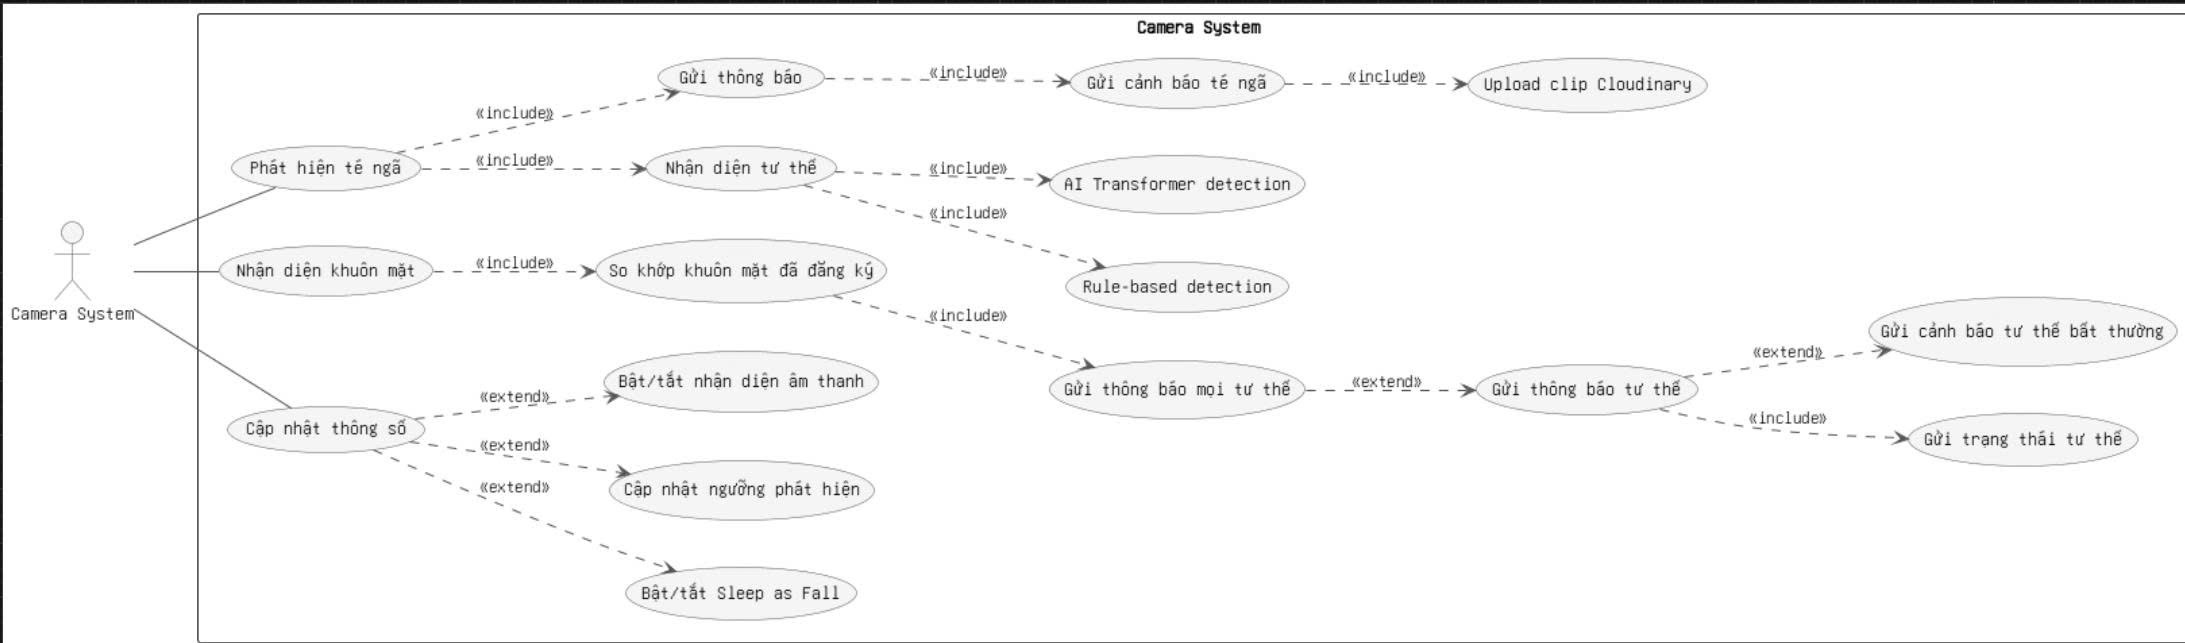
\includegraphics[width=1.0\textwidth]{figures/uc_camera_system.jpg}
    \caption{Sơ đồ Use Case  chi tiết camera system}
    \label{fig:usecase_camera_system}
\end{figure}


\subsection*{UC06 -- Phát hiện té ngã}
\begin{table}[H]
        \captionsetup{justification=raggedright, singlelinecheck=false}
        \caption{Đặc tả UC06 -- Phát hiện té ngã}
\centering
\begin{tabular}{|p{3.5cm}|p{10cm}|}
\hline
\textbf{Tên use case} & Phát hiện té ngã \\
\hline
\textbf{Actor} & Camera System \\
\hline
\textbf{Mô tả} & Hệ thống phát hiện và xác nhận sự kiện
  té ngã, kích hoạt toàn bộ luồng cảnh báo \\
\hline
\textbf{Tiền điều kiện} & Camera đang hoạt động, đã kết nối
  Backend API \\
\hline
\textbf{Hậu điều kiện} & Clip được upload lên Cloudinary,
  cảnh báo được gửi đến người dùng \\
\hline
\textbf{Luồng chính} &
  1. Camera System nhận diện tư thế liên tục \newline
  2. Rule-based và AI Transformer đồng thời xác nhận
     té ngã \newline
  3. Hệ thống cắt clip 6 giây và upload Cloudinary \newline
  4. Hệ thống gửi thông báo đến Backend API \\
\hline
\textbf{Luồng thay thế} &
  2a. Chỉ một cơ chế xác nhận: không kích hoạt
  cảnh báo \newline
  3a. Upload thất bại: gửi thông báo không có clip \\
\hline
\textbf{Include} & Nhận diện tư thế, Gửi thông báo,
  Upload clip Cloudinary \\
\hline
\end{tabular}

\end{table}

\subsection*{UC07 -- Nhận diện tư thế}
\begin{table}[H]
    \captionsetup{justification=raggedright, singlelinecheck=false}
    \caption{Đặc tả UC07 -- Nhận diện tư thế}
\centering
\begin{tabular}{|p{3.5cm}|p{10cm}|}
\hline
\textbf{Tên use case} & Nhận diện tư thế \\
\hline
\textbf{Actor} & Camera System \\
\hline
\textbf{Mô tả} & Hệ thống phân tích frame video để xác định
  tư thế hiện tại của người được giám sát \\
\hline
\textbf{Tiền điều kiện} & Camera đang thu nhận luồng video \\
\hline
\textbf{Hậu điều kiện} & Tư thế được phân loại và cập nhật
  trạng thái hệ thống \\
\hline
\textbf{Luồng chính} &
  1. PoseEngine trích xuất keypoints từ frame \newline
  2. Rule-based detection phân loại tư thế dựa trên
     vận tốc và góc cơ thể \newline
  3. AI Transformer detection xác nhận kết quả với
     độ tin cậy 97,8\% \newline
  4. Hệ thống cập nhật trạng thái tư thế \\
\hline
\textbf{Luồng thay thế} &
  1a. Không phát hiện người: bỏ qua frame \\
\hline
\textbf{Include} & Rule-based detection,
  AI Transformer detection \\
\hline
\end{tabular}
\end{table}

\subsection*{UC08 -- Gửi thông báo}
\begin{table}[H]
    \captionsetup{justification=raggedright, singlelinecheck=false}
    \caption{Đặc tả UC08 -- Gửi thông báo}
\centering
\begin{tabular}{|p{3.5cm}|p{10cm}|}
\hline
\textbf{Tên use case} & Gửi thông báo \\
\hline
\textbf{Actor} & Camera System \\
\hline
\textbf{Mô tả} & Hệ thống gửi thông báo đến Backend API
  để phân phối đến người dùng \\
\hline
\textbf{Tiền điều kiện} & Sự kiện té ngã hoặc tư thế
  đã được xác nhận \\
\hline
\textbf{Hậu điều kiện} & Backend nhận được thông báo
  và phân phối đến người dùng \\
\hline
\textbf{Luồng chính} &
  1. Desktop App gửi sự kiện lên Backend API \newline
  2. Backend phân phối thông báo đến người dùng \\
\hline
\textbf{Luồng thay thế} &
  1a. Mất kết nối Backend: lưu tạm và gửi lại
  khi kết nối được phục hồi \\
\hline
\textbf{Include} & Gửi cảnh báo té ngã \\
\hline
\textbf{Extend} & Gửi thông báo tư thế \\
\hline
\end{tabular}

\end{table}

\subsection*{UC09 -- Gửi cảnh báo té ngã}
\begin{table}[H]
    \captionsetup{justification=raggedright, singlelinecheck=false}
    \caption{Đặc tả UC09 -- Gửi cảnh báo té ngã}
\centering
\begin{tabular}{|p{3.5cm}|p{10cm}|}
\hline
\textbf{Tên use case} & Gửi cảnh báo té ngã \\
\hline
\textbf{Actor} & Camera System \\
\hline
\textbf{Mô tả} & Hệ thống gửi thông tin sự kiện té ngã
  kèm clip video lên Backend API \\
\hline
\textbf{Tiền điều kiện} & Sự kiện té ngã đã được xác nhận,
  clip đã được upload lên Cloudinary \\
\hline
\textbf{Hậu điều kiện} & Backend nhận sự kiện và gửi
  thông báo khẩn cấp đến người dùng \\
\hline
\textbf{Luồng chính} &
  1. Desktop App gọi POST /events/fall \newline
  2. Gửi kèm thông tin vận tốc, góc cơ thể,
     clip\_url và thời gian xảy ra \newline
  3. Backend lưu sự kiện và phân phối thông báo \\
\hline
\textbf{Luồng thay thế} &
  1a. Backend không phản hồi: thử lại tối đa
  3 lần \\
\hline
\textbf{Include từ} & Gửi thông báo \\
\hline
\end{tabular}

\end{table}

\subsection*{UC10 -- Gửi thông báo tư thế}
\begin{table}[H]
    \captionsetup{justification=raggedright, singlelinecheck=false}
    \caption{Đặc tả UC10 -- Gửi thông báo tư thế}
\centering
\begin{tabular}{|p{3.5cm}|p{10cm}|}
\hline
\textbf{Tên use case} & Gửi thông báo tư thế \\
\hline
\textbf{Actor} & Camera System \\
\hline
\textbf{Mô tả} & Hệ thống gửi cập nhật trạng thái tư thế
  của người được giám sát lên Backend theo thời gian thực \\
\hline
\textbf{Tiền điều kiện} & Khuôn mặt người giám sát đã được
  nhận diện \\
\hline
\textbf{Hậu điều kiện} & Trạng thái tư thế được cập nhật
  trên ứng dụng người dùng \\
\hline
\textbf{Luồng chính} &
  1. Hệ thống gửi trạng thái tư thế hiện tại \newline
  2. Backend phân phối cập nhật đến người dùng \\
\hline
\textbf{Luồng thay thế} &
  1a. Tư thế bất thường: gửi cảnh báo tư thế
  bất thường \\
\hline
\textbf{Extend từ} & Gửi thông báo \\
\hline
\textbf{Include} & Gửi trạng thái tư thế \\
\hline
\textbf{Extend} & Gửi cảnh báo tư thế bất thường \\
\hline
\end{tabular}
\end{table}

\subsection*{UC11 -- Nhận diện khuôn mặt}
\begin{table}[H]
    \captionsetup{justification=raggedright, singlelinecheck=false}
    \caption{Đặc tả UC11 -- Nhận diện khuôn mặt}
\centering
\begin{tabular}{|p{3.5cm}|p{10cm}|}
\hline
\textbf{Tên use case} & Nhận diện khuôn mặt \\
\hline
\textbf{Actor} & Camera System \\
\hline
\textbf{Mô tả} & Hệ thống nhận diện và xác định danh tính
  người xuất hiện trong khung hình \\
\hline
\textbf{Tiền điều kiện} & Tính năng nhận diện khuôn mặt
  đã được bật, có khuôn mặt đã đăng ký \\
\hline
\textbf{Hậu điều kiện} & Danh tính người được xác định,
  thông báo tư thế được gửi theo người đó \\
\hline
\textbf{Luồng chính} &
  1. FaceEngine phát hiện khuôn mặt trong frame \newline
  2. Hệ thống so khớp với danh sách khuôn mặt
     đã đăng ký \newline
  3. Xác định danh tính người được giám sát \newline
  4. Gửi thông báo mọi tư thế của người đó \\
\hline
\textbf{Luồng thay thế} &
  2a. Không khớp khuôn mặt: không gửi thông báo
  tư thế \newline
  1a. Không phát hiện khuôn mặt: bỏ qua frame \\
\hline
\textbf{Include} & So khớp khuôn mặt đã đăng ký \\
\hline
\textbf{Extend} & Gửi thông báo mọi tư thế \\
\hline
\end{tabular}
\end{table}

\subsection*{UC12 -- Cập nhật thông số}
\begin{table}[H]
    \captionsetup{justification=raggedright, singlelinecheck=false}
    \caption{Đặc tả UC12 -- Cập nhật thông số}
\centering
\begin{tabular}{|p{3.5cm}|p{10cm}|}
\hline
\textbf{Tên use case} & Cập nhật thông số \\
\hline
\textbf{Actor} & Camera System \\
\hline
\textbf{Mô tả} & Hệ thống nhận và áp dụng các thông số
  cấu hình mới từ Backend \\
\hline
\textbf{Tiền điều kiện} & Desktop App đang kết nối
  Backend API \\
\hline
\textbf{Hậu điều kiện} & Thông số mới được áp dụng
  ngay lập tức \\
\hline
\textbf{Luồng chính} &
  1. Backend gửi cấu hình mới xuống Desktop App \newline
  2. Desktop App nhận và cập nhật thông số \newline
  3. Hệ thống áp dụng thông số mới vào pipeline
     phát hiện \\
\hline
\textbf{Luồng thay thế} &
  1a. Mất kết nối: giữ nguyên thông số cũ \\
\hline
\textbf{Extend} & Bật/tắt Sleep as Fall,
  Cập nhật ngưỡng phát hiện,
  Bật/tắt nhận diện âm thanh \\
\hline
\end{tabular}

\end{table}




\subsection{Sơ đồ Use Case chi tiết xem lịch sử}
\begin{figure}[H]
    \centering
    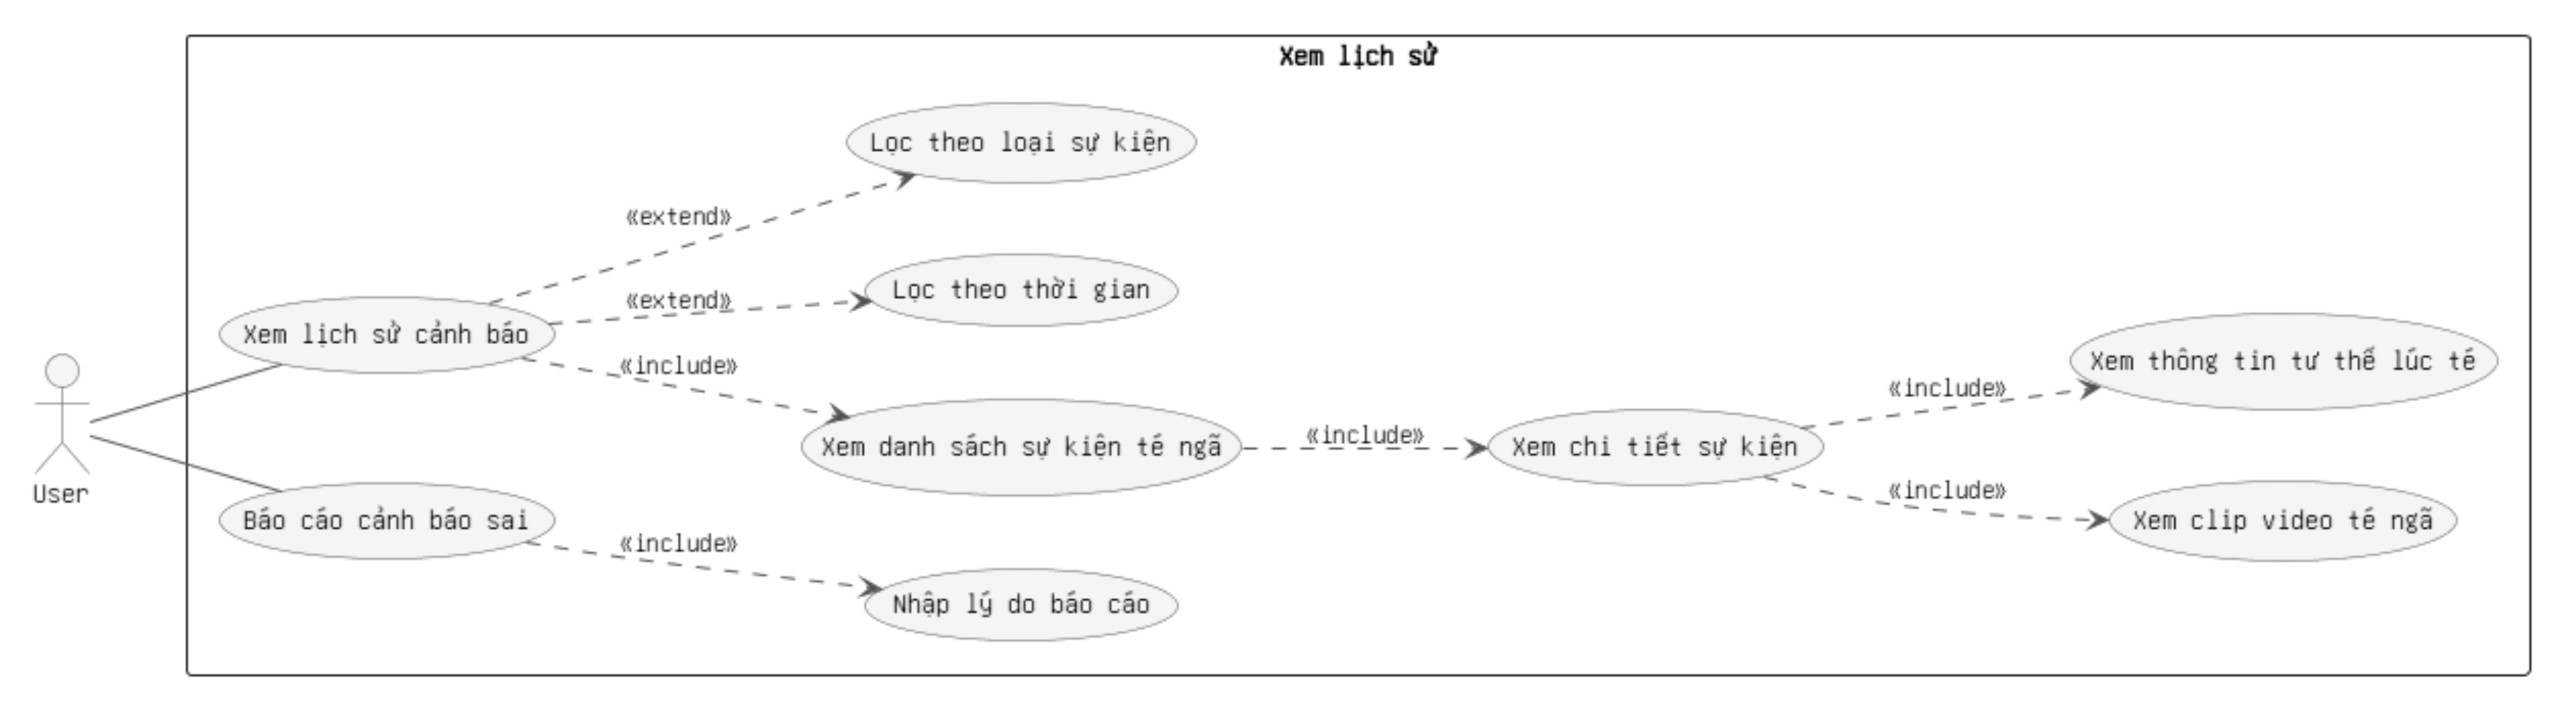
\includegraphics[width=1.0\textwidth]{figures/uc_xem_ls.jpg}
    \caption{Sơ đồ Use Case  chi tiết xem lịch sử}
    \label{fig:usecase_xem_ls}
\end{figure}



\subsection*{UC13 -- Xem lịch sử cảnh báo}
\begin{table}[H]
    \captionsetup{justification=raggedright, singlelinecheck=false}
    \caption{Đặc tả UC13 -- Xem lịch sử cảnh báo}
\centering
\begin{tabular}{|p{3.5cm}|p{10cm}|}
\hline
\textbf{Tên use case} & Xem lịch sử cảnh báo \\
\hline
\textbf{Actor} & User \\
\hline
\textbf{Mô tả} & Người dùng xem toàn bộ danh sách sự kiện
  té ngã đã được ghi nhận \\
\hline
\textbf{Tiền điều kiện} & Người dùng đã đăng nhập \\
\hline
\textbf{Hậu điều kiện} & Danh sách sự kiện được hiển thị \\
\hline
\textbf{Luồng chính} &
  1. Người dùng mở màn hình Lịch sử \newline
  2. Hệ thống gọi GET /events/falls lấy danh sách \newline
  3. Hiển thị danh sách sự kiện té ngã \newline
  4. Người dùng chọn sự kiện để xem chi tiết \\
\hline
\textbf{Luồng thay thế} &
  2a. Chưa có sự kiện: hiển thị thông báo trống \\
\hline
\textbf{Include} & Xem danh sách sự kiện té ngã \\
\hline
\textbf{Extend} & Lọc theo loại sự kiện, Lọc theo thời gian \\
\hline
\end{tabular}

\end{table}

\subsection*{UC14 -- Lọc theo loại sự kiện}
\begin{table}[H]
    \captionsetup{justification=raggedright, singlelinecheck=false}
    \caption{Đặc tả UC14 -- Lọc theo loại sự kiện}
\centering
\begin{tabular}{|p{3.5cm}|p{10cm}|}
\hline
\textbf{Tên use case} & Lọc theo loại sự kiện \\
\hline
\textbf{Actor} & User \\
\hline
\textbf{Mô tả} & Người dùng lọc danh sách sự kiện theo
  loại cảnh báo \\
\hline
\textbf{Tiền điều kiện} & Đang ở màn hình Lịch sử \\
\hline
\textbf{Hậu điều kiện} & Danh sách được lọc theo loại
  đã chọn \\
\hline
\textbf{Luồng chính} &
  1. Người dùng chọn bộ lọc loại sự kiện \newline
  2. Hệ thống gọi API với tham số loại sự kiện \newline
  3. Hiển thị danh sách đã lọc \\
\hline
\textbf{Luồng thay thế} &
  3a. Không có kết quả: hiển thị thông báo trống \\
\hline
\textbf{Extend từ} & Xem lịch sử cảnh báo \\
\hline
\end{tabular}

\end{table}

\subsection*{UC15 -- Lọc theo thời gian}
\begin{table}[H]
    \captionsetup{justification=raggedright, singlelinecheck=false}
    \caption{Đặc tả UC15 -- Lọc theo thời gian}
\centering
\begin{tabular}{|p{3.5cm}|p{10cm}|}
\hline
\textbf{Tên use case} & Lọc theo thời gian \\
\hline
\textbf{Actor} & User \\
\hline
\textbf{Mô tả} & Người dùng lọc danh sách sự kiện theo
  khoảng thời gian \\
\hline
\textbf{Tiền điều kiện} & Đang ở màn hình Lịch sử \\
\hline
\textbf{Hậu điều kiện} & Danh sách được lọc theo khoảng
  thời gian đã chọn \\
\hline
\textbf{Luồng chính} &
  1. Người dùng chọn ngày bắt đầu và ngày kết thúc \newline
  2. Hệ thống gọi API với tham số from và to \newline
  3. Hiển thị danh sách trong khoảng thời gian đó \\
\hline
\textbf{Luồng thay thế} &
  1a. Ngày kết thúc nhỏ hơn ngày bắt đầu: thông báo lỗi \\
\hline
\textbf{Extend từ} & Xem lịch sử cảnh báo \\
\hline
\end{tabular}

\end{table}

\subsection*{UC16 -- Xem danh sách sự kiện té ngã}
\begin{table}[H]
    \captionsetup{justification=raggedright, singlelinecheck=false}
    \caption{Đặc tả UC16 -- Xem danh sách sự kiện té ngã}
\centering
\begin{tabular}{|p{3.5cm}|p{10cm}|}
\hline
\textbf{Tên use case} & Xem danh sách sự kiện té ngã \\
\hline
\textbf{Actor} & User \\
\hline
\textbf{Mô tả} & Hệ thống hiển thị danh sách toàn bộ
  sự kiện té ngã kèm thông tin tóm tắt \\
\hline
\textbf{Tiền điều kiện} & Người dùng đang ở màn hình
  Lịch sử \\
\hline
\textbf{Hậu điều kiện} & Danh sách hiển thị thời gian,
  trạng thái và thumbnail clip \\
\hline
\textbf{Luồng chính} &
  1. Hệ thống gọi GET /events/falls \newline
  2. Hiển thị danh sách có phân trang \newline
  3. Người dùng cuộn để tải thêm \\
\hline
\textbf{Luồng thay thế} &
  1a. Lỗi kết nối: hiển thị thông báo lỗi \\
\hline
\textbf{Include từ} & Xem lịch sử cảnh báo \\
\hline
\textbf{Include} & Xem chi tiết sự kiện \\
\hline
\end{tabular}

\end{table}

\subsection*{UC17 -- Xem chi tiết sự kiện}
\begin{table}[H]
    \captionsetup{justification=raggedright, singlelinecheck=false}
    \caption{Đặc tả UC17 -- Xem chi tiết sự kiện}
\centering
\begin{tabular}{|p{3.5cm}|p{10cm}|}
\hline
\textbf{Tên use case} & Xem chi tiết sự kiện \\
\hline
\textbf{Actor} & User \\
\hline
\textbf{Mô tả} & Người dùng xem đầy đủ thông tin của một
  sự kiện té ngã cụ thể \\
\hline
\textbf{Tiền điều kiện} & Người dùng đã chọn sự kiện từ
  danh sách \\
\hline
\textbf{Hậu điều kiện} & Thông tin chi tiết và clip video
  được hiển thị \\
\hline
\textbf{Luồng chính} &
  1. Người dùng chọn sự kiện \newline
  2. Hệ thống gọi GET /events/falls/\{id\} \newline
  3. Hiển thị thông tin tư thế, vận tốc, thời gian \newline
  4. Tải và phát clip video từ Cloudinary \\
\hline
\textbf{Luồng thay thế} &
  4a. Không có clip\_url: hiển thị thông báo
  không có video \\
\hline
\textbf{Include từ} & Xem danh sách sự kiện té ngã \\
\hline
\textbf{Include} & Xem thông tin tư thế lúc té,
  Xem clip video té ngã \\
\hline
\end{tabular}

\end{table}

\subsection*{UC18 -- Báo cáo cảnh báo sai}
\begin{table}[H]
    \captionsetup{justification=raggedright, singlelinecheck=false}
    \caption{Đặc tả UC18 -- Báo cáo cảnh báo sai}
\centering
\begin{tabular}{|p{3.5cm}|p{10cm}|}
\hline
\textbf{Tên use case} & Báo cáo cảnh báo sai \\
\hline
\textbf{Actor} & User \\
\hline
\textbf{Mô tả} & Người dùng báo cáo sự kiện bị nhận diện
  sai để cải thiện hệ thống \\
\hline
\textbf{Tiền điều kiện} & Người dùng đang xem chi tiết
  sự kiện \\
\hline
\textbf{Hậu điều kiện} & Báo cáo được lưu vào database,
  sự kiện được đánh dấu là\_false\_alarm \\
\hline
\textbf{Luồng chính} &
  1. Người dùng bấm Báo cáo sai \newline
  2. Hệ thống hiển thị form nhập lý do \newline
  3. Người dùng nhập lý do và xác nhận \newline
  4. Hệ thống gọi POST /events/falls/\{id\}/report \newline
  5. Cập nhật trạng thái sự kiện \\
\hline
\textbf{Luồng thay thế} &
  3a. Người dùng hủy: đóng form, không lưu \\
\hline
\textbf{Include} & Nhập lý do báo cáo \\
\hline
\end{tabular}

\end{table}

\subsection{Sơ đồ Use Case chi tiết tùy chỉnh camera}
\begin{figure}[H]
    \centering
    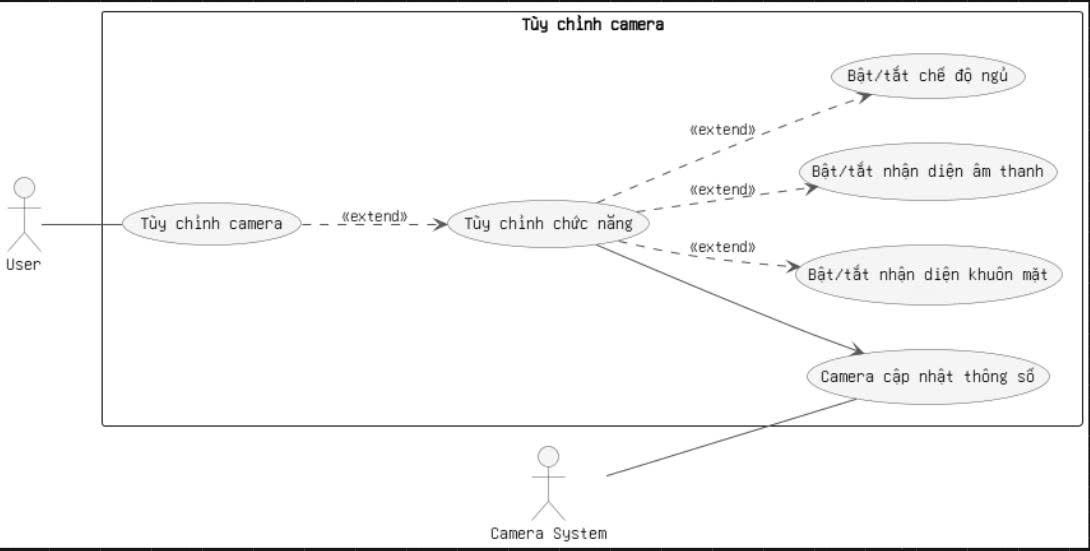
\includegraphics[width=1.0\textwidth]{figures/uc_config.jpg}
    \caption{Sơ đồ Use Case  chi tiết tùy chỉnh camera}
    \label{fig:usecase_tuy_chinh_camera}
\end{figure}

\subsection*{UC19 -- Tùy chỉnh camera}
\begin{table}[H]
    \captionsetup{justification=raggedright, singlelinecheck=false}
    \caption{Đặc tả UC19 -- Tùy chỉnh camera}
\centering
\begin{tabular}{|p{3.5cm}|p{10cm}|}
\hline
\textbf{Tên use case} & Tùy chỉnh camera \\
\hline
\textbf{Actor} & User \\
\hline
\textbf{Mô tả} & Người dùng cấu hình các chức năng hoạt
  động của camera giám sát \\
\hline
\textbf{Tiền điều kiện} & Người dùng đã đăng nhập, camera
  đang kết nối Backend \\
\hline
\textbf{Hậu điều kiện} & Cấu hình mới được lưu và áp dụng
  ngay lập tức cho camera \\
\hline
\textbf{Luồng chính} &
  1. Người dùng mở màn hình Tùy chỉnh camera \newline
  2. Hệ thống hiển thị cấu hình hiện tại từ Backend \newline
  3. Người dùng thay đổi các chức năng mong muốn \newline
  4. Hệ thống lưu và đồng bộ cấu hình với camera \\
\hline
\textbf{Luồng thay thế} &
  4a. Camera offline: lưu DB, áp dụng khi camera
  kết nối lại \\
\hline
\textbf{Extend} & Tùy chỉnh chức năng \\
\hline
\end{tabular}

\end{table}

\subsection*{UC20 -- Tùy chỉnh chức năng}
\begin{table}[H]
    \captionsetup{justification=raggedright, singlelinecheck=false}
    \caption{Đặc tả UC20 -- Tùy chỉnh chức năng}
\centering
\begin{tabular}{|p{3.5cm}|p{10cm}|}
\hline
\textbf{Tên use case} & Tùy chỉnh chức năng \\
\hline
\textbf{Actor} & User \\
\hline
\textbf{Mô tả} & Người dùng bật hoặc tắt các tính năng
  của camera giám sát \\
\hline
\textbf{Tiền điều kiện} & Đang ở màn hình Tùy chỉnh camera \\
\hline
\textbf{Hậu điều kiện} & Trạng thái tính năng được cập nhật
  và camera áp dụng ngay lập tức \\
\hline
\textbf{Luồng chính} &
  1. Người dùng xem danh sách tính năng hiện tại \newline
  2. Người dùng bật hoặc tắt tính năng mong muốn \newline
  3. Hệ thống lưu và gửi cấu hình mới đến camera \\
\hline
\textbf{Luồng thay thế} &
  3a. Lỗi kết nối: thông báo cập nhật thất bại \\
\hline
\textbf{Extend từ} & Tùy chỉnh camera \\
\hline
\textbf{Extend} & Bật/tắt nhận diện khuôn mặt,
  Bật/tắt chế độ ngủ,
  Bật/tắt nhận diện âm thanh \\
\hline
\end{tabular}

\end{table}

\subsection*{UC21 -- Camera cập nhật thông số}
\begin{table}[H]
    \captionsetup{justification=raggedright, singlelinecheck=false}
    \caption{Đặc tả UC21 -- Camera cập nhật thông số}
\centering
\begin{tabular}{|p{3.5cm}|p{10cm}|}
\hline
\textbf{Tên use case} & Camera cập nhật thông số \\
\hline
\textbf{Actor} & Camera System \\
\hline
\textbf{Mô tả} & Camera nhận cấu hình mới từ Backend và
  áp dụng ngay lập tức mà không cần khởi động lại \\
\hline
\textbf{Tiền điều kiện} & Camera đang kết nối Backend,
  có thông số mới từ người dùng \\
\hline
\textbf{Hậu điều kiện} & Thông số mới được áp dụng cho
  pipeline phát hiện \\
\hline
\textbf{Luồng chính} &
  1. Backend gửi cấu hình mới xuống Desktop App \newline
  2. Camera nhận thông số cấu hình mới \newline
  3. Pipeline phát hiện cập nhật cấu hình \newline
  4. Camera xác nhận đã áp dụng thành công \\
\hline
\textbf{Luồng thay thế} &
  1a. Mất kết nối: lấy cấu hình mới khi kết nối lại \\
\hline
\textbf{Include từ} & Tùy chỉnh chức năng \\
\hline
\end{tabular}

\end{table}


\subsection{Sơ đồ Use Case chi tiết cài đặt theo dõi}
\begin{figure}[H]
    \centering
    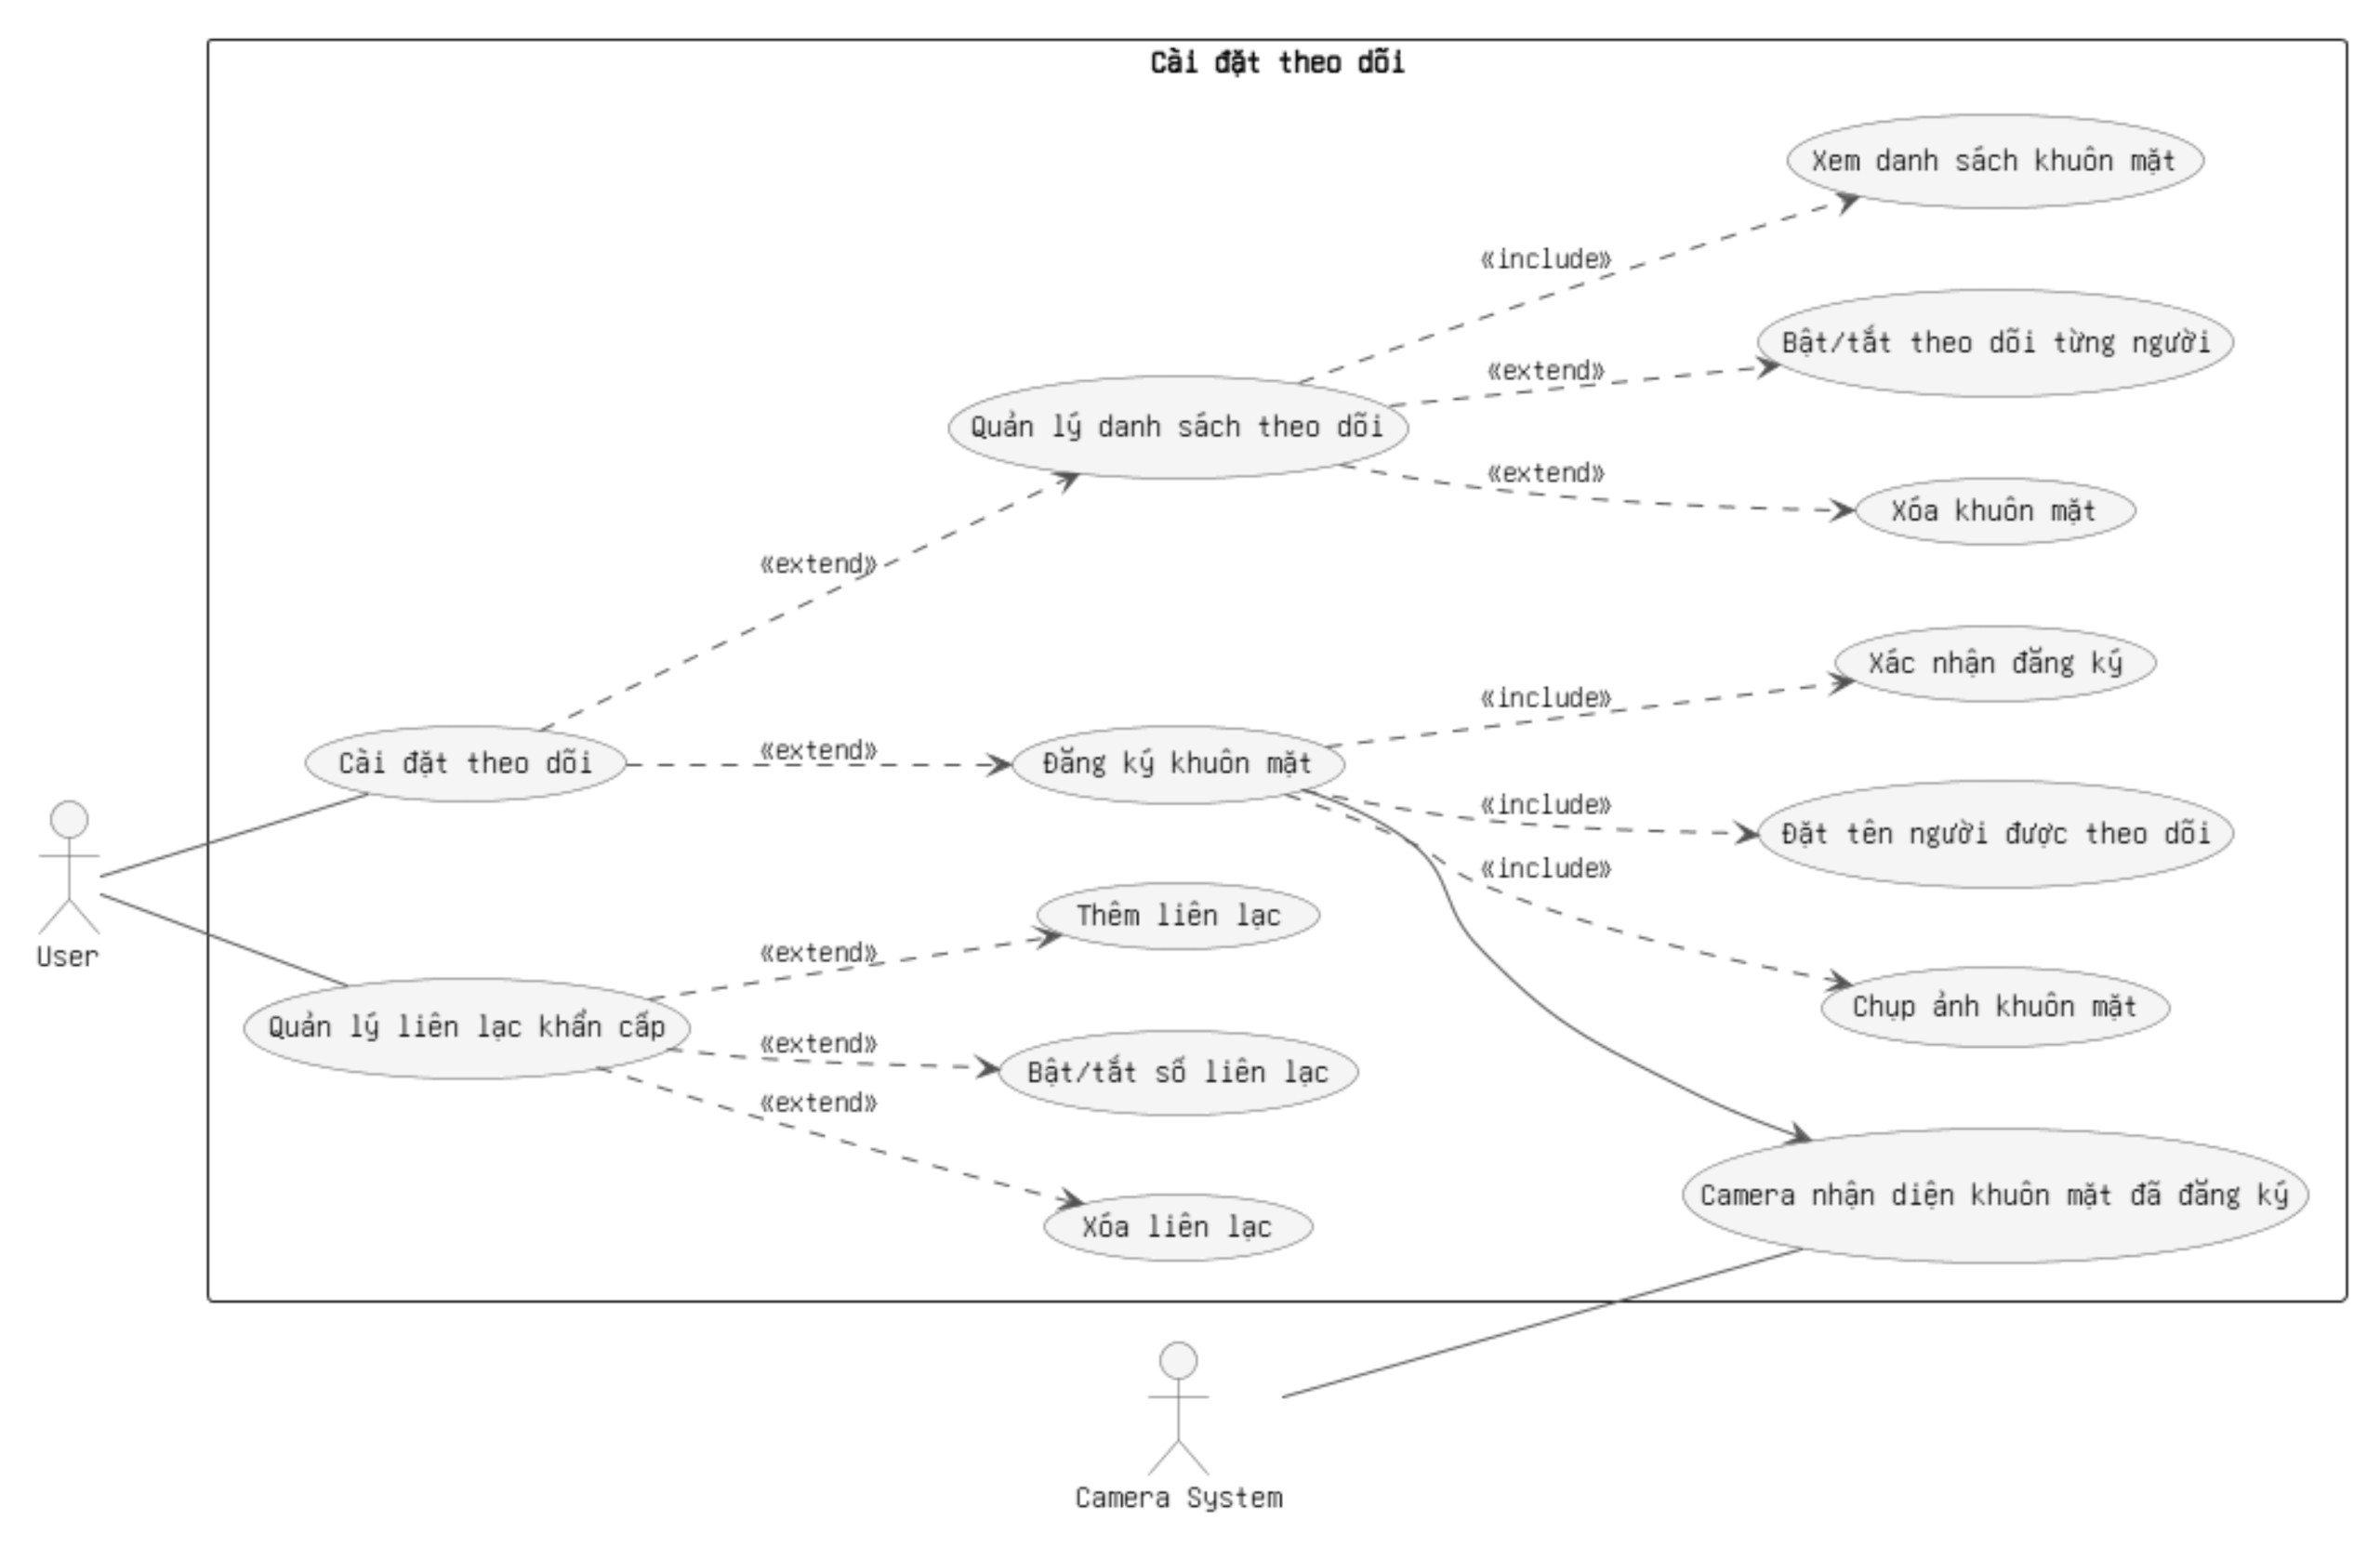
\includegraphics[width=1.0\textwidth]{figures/uc_cai_dat_theo_doi.jpg}
    \caption{Sơ đồ Use Case  chi tiết cài đặt theo dõi}
    \label{fig:usecase_cai_dat_theo_doi}
\end{figure}


\subsection*{UC22 -- Cài đặt theo dõi}
\begin{table}[H]
    \captionsetup{justification=raggedright, singlelinecheck=false}
    \caption{Đặc tả UC22 -- Cài đặt theo dõi}
\centering
\begin{tabular}{|p{3.5cm}|p{10cm}|}
\hline
\textbf{Tên use case} & Cài đặt theo dõi \\
\hline
\textbf{Actor} & User \\
\hline
\textbf{Mô tả} & Người dùng cấu hình thông tin người cần
  giám sát và số liên hệ khẩn cấp \\
\hline
\textbf{Tiền điều kiện} & Người dùng đã đăng nhập \\
\hline
\textbf{Hậu điều kiện} & Thông tin theo dõi được lưu,
  camera cập nhật danh sách nhận diện \\
\hline
\textbf{Luồng chính} &
  1. Người dùng mở màn hình Cài đặt theo dõi \newline
  2. Hệ thống hiển thị danh sách khuôn mặt và
     số liên hệ hiện tại \newline
  3. Người dùng thực hiện các thao tác quản lý \\
\hline
\textbf{Luồng thay thế} &
  2a. Chưa có dữ liệu: hiển thị giao diện trống \\
\hline
\textbf{Extend} & Quản lý danh sách theo dõi,
  Đăng ký khuôn mặt, Quản lý liên lạc khẩn cấp \\
\hline
\end{tabular}

\end{table}

\subsection*{UC23 -- Quản lý danh sách theo dõi}
\begin{table}[H]
    \captionsetup{justification=raggedright, singlelinecheck=false}
    \caption{Đặc tả UC23 -- Quản lý danh sách theo dõi}
\centering
\begin{tabular}{|p{3.5cm}|p{10cm}|}
\hline
\textbf{Tên use case} & Quản lý danh sách theo dõi \\
\hline
\textbf{Actor} & User \\
\hline
\textbf{Mô tả} & Người dùng quản lý danh sách khuôn mặt
  người cần giám sát \\
\hline
\textbf{Tiền điều kiện} & Người dùng đang ở màn hình
  Cài đặt theo dõi \\
\hline
\textbf{Hậu điều kiện} & Danh sách khuôn mặt được cập nhật \\
\hline
\textbf{Luồng chính} &
  1. Hệ thống hiển thị danh sách khuôn mặt đã đăng ký \newline
  2. Người dùng thực hiện bật/tắt hoặc xóa khuôn mặt \newline
  3. Hệ thống cập nhật và đồng bộ với camera \\
\hline
\textbf{Luồng thay thế} &
  2a. Xóa khuôn mặt: xác nhận trước khi xóa \\
\hline
\textbf{Extend từ} & Cài đặt theo dõi \\
\hline
\textbf{Include} & Xem danh sách khuôn mặt \\
\hline
\textbf{Extend} & Bật/tắt theo dõi từng người, Xóa khuôn mặt \\
\hline
\end{tabular}

\end{table}

\subsection*{UC24 -- Đăng ký khuôn mặt}
\begin{table}[H]
    \captionsetup{justification=raggedright, singlelinecheck=false}
    \caption{Đặc tả UC24 -- Đăng ký khuôn mặt}
\centering
\begin{tabular}{|p{3.5cm}|p{10cm}|}
\hline
\textbf{Tên use case} & Đăng ký khuôn mặt \\
\hline
\textbf{Actor} & User, Camera System \\
\hline
\textbf{Mô tả} & Người dùng đăng ký khuôn mặt người cần
  giám sát để camera nhận diện và theo dõi tư thế \\
\hline
\textbf{Tiền điều kiện} & Camera đang hoạt động, người
  cần đăng ký đứng trước camera \\
\hline
\textbf{Hậu điều kiện} & Khuôn mặt được lưu vào DB,
  camera bắt đầu nhận diện người này \\
\hline
\textbf{Luồng chính} &
  1. Người dùng chọn Đăng ký khuôn mặt \newline
  2. Camera chụp ảnh khuôn mặt \newline
  3. Người dùng đặt tên người được theo dõi \newline
  4. Hệ thống trích xuất face embedding \newline
  5. Lưu vào DB và cập nhật danh sách nhận diện camera \newline
  6. Người dùng xác nhận đăng ký thành công \\
\hline
\textbf{Luồng thay thế} &
  2a. Không phát hiện khuôn mặt: yêu cầu chụp lại \newline
  5a. Lỗi lưu DB: thông báo thất bại \\
\hline
\textbf{Extend từ} & Cài đặt theo dõi \\
\hline
\textbf{Include} & Chụp ảnh khuôn mặt, Đặt tên người
  được theo dõi, Xác nhận đăng ký \\
\hline
\end{tabular}

\end{table}

\subsection*{UC25 -- Quản lý liên lạc khẩn cấp}
\begin{table}[H]
    \captionsetup{justification=raggedright, singlelinecheck=false}
    \caption{Đặc tả UC25 -- Quản lý liên lạc khẩn cấp}
\centering
\begin{tabular}{|p{3.5cm}|p{10cm}|}
\hline
\textbf{Tên use case} & Quản lý liên lạc khẩn cấp \\
\hline
\textbf{Actor} & User \\
\hline
\textbf{Mô tả} & Người dùng quản lý danh sách số điện
  thoại nhận cảnh báo khi phát hiện té ngã \\
\hline
\textbf{Tiền điều kiện} & Người dùng đã đăng nhập \\
\hline
\textbf{Hậu điều kiện} & Danh sách liên lạc được cập nhật,
  hệ thống áp dụng khi có sự kiện té ngã \\
\hline
\textbf{Luồng chính} &
  1. Hệ thống hiển thị danh sách số liên lạc hiện tại \newline
  2. Người dùng thêm, bật/tắt hoặc xóa số liên lạc \newline
  3. Hệ thống lưu thay đổi vào DB \\
\hline
\textbf{Luồng thay thế} &
  2a. Thêm quá 5 số: thông báo đã đạt giới hạn \newline
  2b. Số điện thoại không đúng định dạng VN:
  thông báo lỗi \\
\hline
\textbf{Extend từ} & Cài đặt theo dõi \\
\hline
\textbf{Extend} & Thêm liên lạc, Bật/tắt số liên lạc,
  Xóa liên lạc \\
\hline
\end{tabular}

\end{table}

\subsection*{UC26 -- Camera nhận diện khuôn mặt đã đăng ký}
\begin{table}[H]
    \captionsetup{justification=raggedright, singlelinecheck=false}
    \caption{Đặc tả UC26 -- Camera nhận diện khuôn mặt đã đăng ký}
\centering
\begin{tabular}{|p{3.5cm}|p{10cm}|}
\hline
\textbf{Tên use case} & Camera nhận diện khuôn mặt
  đã đăng ký \\
\hline
\textbf{Actor} & Camera System \\
\hline
\textbf{Mô tả} & Camera tự động nhận diện người đã đăng ký
  và theo dõi mọi tư thế, chỉ gọi điện và SMS khi té ngã \\
\hline
\textbf{Tiền điều kiện} & Có ít nhất một khuôn mặt đã
  đăng ký trong DB \\
\hline
\textbf{Hậu điều kiện} & Tư thế người được theo dõi liên
  tục, thông báo tư thế được gửi đến người dùng \\
\hline
\textbf{Luồng chính} &
  1. Camera phát hiện khuôn mặt trong khung hình \newline
  2. So khớp với danh sách khuôn mặt đã đăng ký \newline
  3. Xác nhận danh tính, bắt đầu theo dõi tư thế \newline
  4. Gửi thông báo tư thế realtime qua WebSocket \newline
  5. Nếu phát hiện té ngã: kích hoạt gọi điện và SMS \\
\hline
\textbf{Luồng thay thế} &
  2a. Không khớp: tiếp tục giám sát bình thường \newline
  5a. Không có số liên lạc: bỏ qua gọi và SMS \\
\hline
\textbf{Trigger từ} & Đăng ký khuôn mặt \\
\hline
\end{tabular}

\end{table}


\subsection{Sơ đồ Use Case chi tiết xử lý thông báo}
\begin{figure}[H]
    \centering
    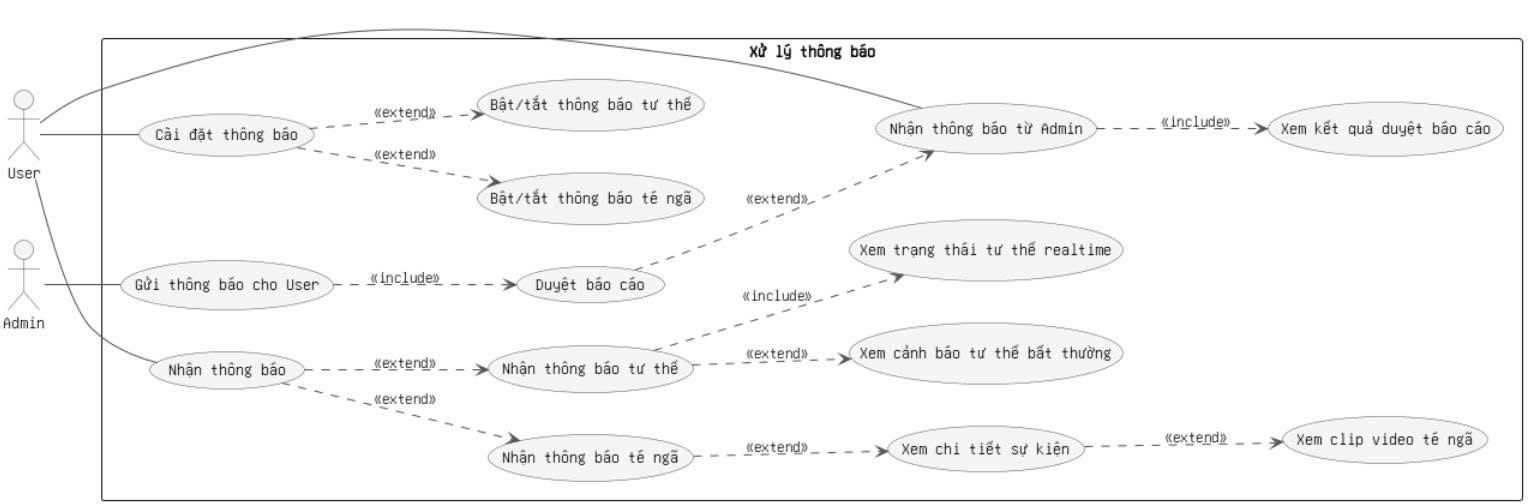
\includegraphics[width=1.0\textwidth]{figures/uc_thong_bao.jpg}
    \caption{Sơ đồ Use Case  chi tiết xử lý thông báo}
    \label{fig:usecase_xu_ly_thong_bao}
\end{figure}
\subsection*{UC27 -- Nhận thông báo}
\begin{table}[H]
    \captionsetup{justification=raggedright, singlelinecheck=false}
    \caption{Đặc tả UC27 -- Nhận thông báo}
\centering
\begin{tabular}{|p{3.5cm}|p{10cm}|}
\hline
\textbf{Tên use case} & Nhận thông báo \\
\hline
\textbf{Actor} & User \\
\hline
\textbf{Mô tả} & Người dùng nhận và xử lý các loại thông
  báo từ hệ thống và từ Admin \\
\hline
\textbf{Tiền điều kiện} & Người dùng đã đăng nhập, ứng dụng
  đang chạy hoặc nền \\
\hline
\textbf{Hậu điều kiện} & Thông báo được hiển thị đến
  người dùng \\
\hline
\textbf{Luồng chính} &
  1. Hệ thống phát sinh sự kiện té ngã, tư thế bất thường
     hoặc Admin gửi thông báo \newline
  2. Backend gửi thông báo đến thiết bị người dùng \newline
  3. Người dùng nhận và xem thông báo \\
\hline
\textbf{Luồng thay thế} &
  2a. Ứng dụng đang tắt: thông báo hiển thị
  trên thanh thông báo hệ thống \\
\hline
\textbf{Extend} & Nhận thông báo té ngã,
  Nhận thông báo tư thế,
  Nhận thông báo từ Admin \\
\hline
\end{tabular}

\end{table}

\subsection*{UC28 -- Nhận thông báo té ngã}
\begin{table}[H]
    \captionsetup{justification=raggedright, singlelinecheck=false}
    \caption{Đặc tả UC28 -- Nhận thông báo té ngã}
\centering
\begin{tabular}{|p{3.5cm}|p{10cm}|}
\hline
\textbf{Tên use case} & Nhận thông báo té ngã \\
\hline
\textbf{Actor} & User \\
\hline
\textbf{Mô tả} & Người dùng nhận cảnh báo khẩn cấp khi
  hệ thống phát hiện sự kiện té ngã \\
\hline
\textbf{Tiền điều kiện} & Hệ thống đã xác nhận sự kiện
  té ngã \\
\hline
\textbf{Hậu điều kiện} & Người dùng nhận được thông báo
  và có thể xem chi tiết sự kiện \\
\hline
\textbf{Luồng chính} &
  1. Camera System phát hiện té ngã, gửi lên Backend \newline
  2. Backend gửi FCM push đến thiết bị người dùng \newline
  3. Thông báo hiển thị trên màn hình điện thoại \newline
  4. Người dùng bấm vào thông báo để xem chi tiết \\
\hline
\textbf{Luồng thay thế} &
  3a. Người dùng không bấm vào: thông báo
  lưu trong danh sách lịch sử \\
\hline
\textbf{Extend từ} & Nhận thông báo \\
\hline
\textbf{Extend} & Xem chi tiết sự kiện \\
\hline
\end{tabular}

\end{table}

\subsection*{UC29 -- Xem chi tiết sự kiện}
\begin{table}[H]
    \captionsetup{justification=raggedright, singlelinecheck=false}
    \caption{Đặc tả UC29 -- Xem chi tiết sự kiện}
\centering
\begin{tabular}{|p{3.5cm}|p{10cm}|}
\hline
\textbf{Tên use case} & Xem chi tiết sự kiện \\
\hline
\textbf{Actor} & User \\
\hline
\textbf{Mô tả} & Người dùng bấm vào thông báo té ngã để
  xem thông tin chi tiết của sự kiện \\
\hline
\textbf{Tiền điều kiện} & Người dùng đã nhận thông báo
  té ngã \\
\hline
\textbf{Hậu điều kiện} & Màn hình chi tiết sự kiện được
  hiển thị với đầy đủ thông tin \\
\hline
\textbf{Luồng chính} &
  1. Người dùng bấm vào thông báo \newline
  2. Ứng dụng mở màn hình chi tiết sự kiện \newline
  3. Hệ thống hiển thị thời gian, camera, vận tốc
     và góc cơ thể \newline
  4. Người dùng có thể xem clip video kèm theo \\
\hline
\textbf{Luồng thay thế} &
  4a. Clip chưa upload xong: hiển thị trạng thái
  đang xử lý \\
\hline
\textbf{Extend từ} & Nhận thông báo té ngã \\
\hline
\textbf{Extend} & Xem clip video té ngã \\
\hline
\end{tabular}

\end{table}

\subsection*{UC30 -- Xem clip video té ngã}
\begin{table}[H]
    \captionsetup{justification=raggedright, singlelinecheck=false}
    \caption{Đặc tả UC30 -- Xem clip video té ngã}
\centering
\begin{tabular}{|p{3.5cm}|p{10cm}|}
\hline
\textbf{Tên use case} & Xem clip video té ngã \\
\hline
\textbf{Actor} & User \\
\hline
\textbf{Mô tả} & Người dùng xem đoạn video 6 giây ghi lại
  sự kiện té ngã từ camera giám sát \\
\hline
\textbf{Tiền điều kiện} & Người dùng đang ở màn hình chi
  tiết sự kiện, clip đã được upload lên Cloudinary \\
\hline
\textbf{Hậu điều kiện} & Video được phát trên màn hình
  điện thoại \\
\hline
\textbf{Luồng chính} &
  1. Người dùng bấm nút xem clip \newline
  2. Ứng dụng tải clip từ đường dẫn Cloudinary \newline
  3. Video player hiển thị và phát clip tự động \\
\hline
\textbf{Luồng thay thế} &
  2a. Không có kết nối mạng: hiển thị thông báo
  lỗi tải video \\
\hline
\textbf{Extend từ} & Xem chi tiết sự kiện \\
\hline
\end{tabular}

\end{table}

\subsection*{UC31 -- Nhận thông báo tư thế}
\begin{table}[H]
    \captionsetup{justification=raggedright, singlelinecheck=false}
    \caption{Đặc tả UC31 -- Nhận thông báo tư thế}
\centering
\begin{tabular}{|p{3.5cm}|p{10cm}|}
\hline
\textbf{Tên use case} & Nhận thông báo tư thế \\
\hline
\textbf{Actor} & User \\
\hline
\textbf{Mô tả} & Người dùng nhận thông báo về trạng thái
  tư thế của người được giám sát theo thời gian thực \\
\hline
\textbf{Tiền điều kiện} & Đã đăng ký khuôn mặt người giám
  sát, tính năng thông báo tư thế đang bật \\
\hline
\textbf{Hậu điều kiện} & Trạng thái tư thế được cập nhật
  trên ứng dụng \\
\hline
\textbf{Luồng chính} &
  1. Camera nhận diện tư thế người đã đăng ký \newline
  2. Backend gửi thông báo cập nhật tư thế \newline
  3. Ứng dụng cập nhật trạng thái tư thế realtime \\
\hline
\textbf{Luồng thay thế} &
  3a. Tư thế bất thường: hiển thị cảnh báo
  tư thế bất thường \\
\hline
\textbf{Extend từ} & Nhận thông báo \\
\hline
\textbf{Include} & Xem trạng thái tư thế realtime \\
\hline
\textbf{Extend} & Xem cảnh báo tư thế bất thường \\
\hline
\end{tabular}

\end{table}

\subsection*{UC32 -- Cài đặt thông báo}
\begin{table}[H]
    \captionsetup{justification=raggedright, singlelinecheck=false}
    \caption{Đặc tả UC32 -- Cài đặt thông báo}
\centering
\begin{tabular}{|p{3.5cm}|p{10cm}|}
\hline
\textbf{Tên use case} & Cài đặt thông báo \\
\hline
\textbf{Actor} & User \\
\hline
\textbf{Mô tả} & Người dùng tùy chỉnh các loại thông báo
  muốn nhận từ hệ thống \\
\hline
\textbf{Tiền điều kiện} & Người dùng đã đăng nhập \\
\hline
\textbf{Hậu điều kiện} & Cấu hình thông báo được lưu
  và áp dụng \\
\hline
\textbf{Luồng chính} &
  1. Người dùng mở màn hình Cài đặt thông báo \newline
  2. Hệ thống hiển thị cấu hình hiện tại \newline
  3. Người dùng bật hoặc tắt từng loại thông báo \newline
  4. Hệ thống lưu cấu hình \\
\hline
\textbf{Luồng thay thế} &
  4a. Lỗi kết nối: thông báo lưu thất bại,
  giữ nguyên cấu hình cũ \\
\hline
\textbf{Extend} & Bật/tắt thông báo té ngã,
  Bật/tắt thông báo tư thế \\
\hline
\end{tabular}

\end{table}

\subsection*{UC33 -- Nhận thông báo từ Admin}
\begin{table}[H]
    \captionsetup{justification=raggedright, singlelinecheck=false}
    \caption{Đặc tả UC33 -- Nhận thông báo từ Admin}
\centering
\begin{tabular}{|p{3.5cm}|p{10cm}|}
\hline
\textbf{Tên use case} & Nhận thông báo từ Admin \\
\hline
\textbf{Actor} & User \\
\hline
\textbf{Mô tả} & Người dùng nhận thông báo kết quả duyệt
  báo cáo sai do Admin gửi \\
\hline
\textbf{Tiền điều kiện} & Người dùng đã gửi báo cáo sai,
  Admin đã thực hiện duyệt báo cáo \\
\hline
\textbf{Hậu điều kiện} & Người dùng biết được kết quả
  xử lý báo cáo của mình \\
\hline
\textbf{Luồng chính} &
  1. Admin duyệt hoặc từ chối báo cáo sai \newline
  2. Backend gửi FCM push đến thiết bị người dùng \newline
  3. Người dùng nhận thông báo và xem kết quả \\
\hline
\textbf{Luồng thay thế} &
  3a. Ứng dụng đang tắt: thông báo hiển thị
  trên thanh thông báo hệ thống \\
\hline
\textbf{Extend từ} & Nhận thông báo \\
\hline
\textbf{Include} & Xem kết quả duyệt báo cáo \\
\hline
\end{tabular}
\end{table}

\subsection*{UC34 -- Gửi thông báo cho User}
\begin{table}[H]
    \captionsetup{justification=raggedright, singlelinecheck=false}
    \caption{Đặc tả UC34 -- Gửi thông báo cho User}
\centering
\begin{tabular}{|p{3.5cm}|p{10cm}|}
\hline
\textbf{Tên use case} & Gửi thông báo cho User \\
\hline
\textbf{Actor} & Admin \\
\hline
\textbf{Mô tả} & Admin gửi thông báo kết quả duyệt báo
  cáo sai đến người dùng liên quan \\
\hline
\textbf{Tiền điều kiện} & Admin đã đăng nhập Web Admin,
  có báo cáo sai chờ xử lý \\
\hline
\textbf{Hậu điều kiện} & Người dùng nhận được thông báo
  kết quả qua FCM \\
\hline
\textbf{Luồng chính} &
  1. Admin xem chi tiết báo cáo sai \newline
  2. Admin chấp nhận hoặc từ chối báo cáo \newline
  3. Hệ thống tự động gửi FCM đến người dùng
     kèm kết quả duyệt \\
\hline
\textbf{Luồng thay thế} &
  3a. Gửi FCM thất bại: hệ thống thử lại,
  thông báo lưu trong lịch sử \\
\hline
\textbf{Include} & Duyệt báo cáo sai \\
\hline
\end{tabular}

\end{table}



\subsection{Sơ đồ Use Case chi tiết quản lý hệ thống- Admin}
\begin{figure}[H]
    \centering
    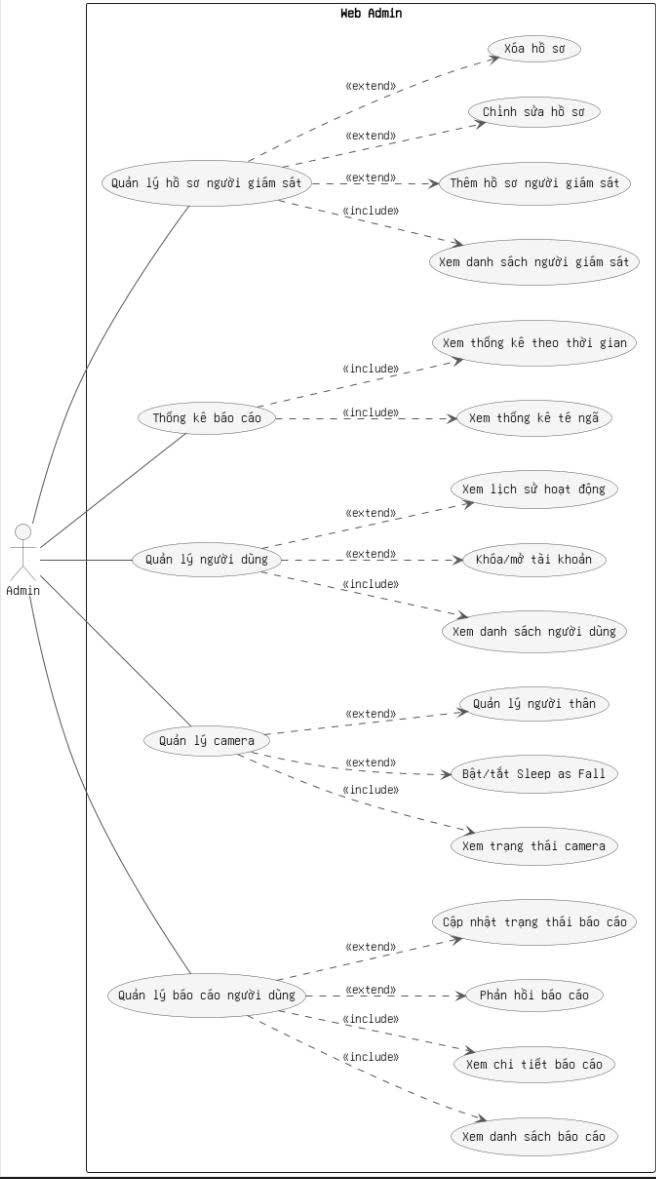
\includegraphics[width=0.7\textwidth]{figures/uc_quanly.jpg}
    \caption{Sơ đồ Use Case  chi tiết quản lý hệ thống- Admin}
    \label{fig:usecase_quan_ly_he_thong}
\end{figure}


\subsection*{UC35 -- Quản lý hồ sơ người giám sát}
\begin{table}[H]
    \captionsetup{justification=raggedright, singlelinecheck=false}
    \caption{Đặc tả UC35 -- Quản lý hồ sơ người giám sát}
\centering
\begin{tabular}{|p{3.5cm}|p{10cm}|}
\hline
\textbf{Tên use case} & Quản lý hồ sơ người giám sát \\
\hline
\textbf{Actor} & Admin \\
\hline
\textbf{Mô tả} & Admin quản lý toàn bộ hồ sơ thông tin
  người được giám sát trong hệ thống \\
\hline
\textbf{Tiền điều kiện} & Admin đã đăng nhập Web Admin \\
\hline
\textbf{Hậu điều kiện} & Thay đổi hồ sơ được lưu vào DB \\
\hline
\textbf{Luồng chính} &
  1. Admin mở màn hình Quản lý hồ sơ \newline
  2. Hệ thống hiển thị danh sách người giám sát \newline
  3. Admin thực hiện thêm, chỉnh sửa hoặc xóa hồ sơ \newline
  4. Hệ thống lưu thay đổi vào DB \\
\hline
\textbf{Luồng thay thế} &
  3a. Xóa hồ sơ: xác nhận trước khi xóa \\
\hline
\textbf{Include} & Xem danh sách người giám sát \\
\hline
\textbf{Extend} & Thêm hồ sơ người giám sát,
  Chỉnh sửa hồ sơ, Xóa hồ sơ \\
\hline
\end{tabular}

\end{table}

\subsection*{UC36 -- Xem danh sách người giám sát}
\begin{table}[H]
    \captionsetup{justification=raggedright, singlelinecheck=false}
    \caption{Đặc tả UC36 -- Xem danh sách người giám sát}
\centering
\begin{tabular}{|p{3.5cm}|p{10cm}|}
\hline
\textbf{Tên use case} & Xem danh sách người giám sát \\
\hline
\textbf{Actor} & Admin \\
\hline
\textbf{Mô tả} & Admin xem toàn bộ danh sách hồ sơ người
  được giám sát kèm thông tin tóm tắt \\
\hline
\textbf{Tiền điều kiện} & Admin đang ở màn hình Quản lý
  hồ sơ \\
\hline
\textbf{Hậu điều kiện} & Danh sách hồ sơ được hiển thị \\
\hline
\textbf{Luồng chính} &
  1. Hệ thống gọi GET /admin/profiles \newline
  2. Hiển thị danh sách có phân trang \newline
  3. Admin có thể tìm kiếm theo tên \\
\hline
\textbf{Luồng thay thế} &
  1a. Chưa có hồ sơ: hiển thị thông báo trống \\
\hline
\textbf{Include từ} & Quản lý hồ sơ người giám sát \\
\hline
\end{tabular}

\end{table}

\subsection*{UC37 -- Thống kê báo cáo}
\begin{table}[H]
    \captionsetup{justification=raggedright, singlelinecheck=false}
    \caption{Đặc tả UC37 -- Thống kê báo cáo}
\centering
\begin{tabular}{|p{3.5cm}|p{10cm}|}
\hline
\textbf{Tên use case} & Thống kê báo cáo \\
\hline
\textbf{Actor} & Admin \\
\hline
\textbf{Mô tả} & Admin xem thống kê tổng quan về hoạt động
  hệ thống \\
\hline
\textbf{Tiền điều kiện} & Admin đã đăng nhập Web Admin \\
\hline
\textbf{Hậu điều kiện} & Dữ liệu thống kê được hiển thị \\
\hline
\textbf{Luồng chính} &
  1. Admin mở màn hình Thống kê \newline
  2. Hệ thống hiển thị thống kê tổng quan \newline
  3. Admin xem chi tiết theo thời gian hoặc
     loại sự kiện \\
\hline
\textbf{Include} & Xem thống kê theo thời gian,
  Xem thống kê té ngã \\
\hline
\end{tabular}

\end{table}

\subsection*{UC38 -- Xem thống kê té ngã}
\begin{table}[H]
    \captionsetup{justification=raggedright, singlelinecheck=false}
    \caption{Đặc tả UC38 -- Xem thống kê té ngã}
\centering
\begin{tabular}{|p{3.5cm}|p{10cm}|}
\hline
\textbf{Tên use case} & Xem thống kê té ngã \\
\hline
\textbf{Actor} & Admin \\
\hline
\textbf{Mô tả} & Admin xem số liệu thống kê về các sự kiện
  té ngã trong hệ thống \\
\hline
\textbf{Tiền điều kiện} & Admin đang ở màn hình Thống kê \\
\hline
\textbf{Hậu điều kiện} & Biểu đồ và số liệu thống kê
  được hiển thị \\
\hline
\textbf{Luồng chính} &
  1. Hệ thống gọi GET /admin/stats/falls \newline
  2. Hiển thị tổng số sự kiện, tỉ lệ nhận diện đúng
     và sai \newline
  3. Hiển thị biểu đồ theo ngày, tuần, tháng \\
\hline
\textbf{Luồng thay thế} &
  1a. Chưa có dữ liệu: hiển thị biểu đồ trống \\
\hline
\textbf{Include từ} & Thống kê báo cáo \\
\hline
\end{tabular}

\end{table}

\subsection*{UC39 -- Quản lý người dùng}
\begin{table}[H]
    \captionsetup{justification=raggedright, singlelinecheck=false}
    \caption{Đặc tả UC39 -- Quản lý người dùng}
\centering
\begin{tabular}{|p{3.5cm}|p{10cm}|}
\hline
\textbf{Tên use case} & Quản lý người dùng \\
\hline
\textbf{Actor} & Admin \\
\hline
\textbf{Mô tả} & Admin quản lý toàn bộ tài khoản người
  dùng trong hệ thống \\
\hline
\textbf{Tiền điều kiện} & Admin đã đăng nhập Web Admin \\
\hline
\textbf{Hậu điều kiện} & Thay đổi tài khoản được lưu vào DB \\
\hline
\textbf{Luồng chính} &
  1. Admin mở màn hình Quản lý người dùng \newline
  2. Hệ thống hiển thị danh sách tài khoản \newline
  3. Admin xem lịch sử hoặc thay đổi trạng thái tài khoản \\
\hline
\textbf{Luồng thay thế} &
  3a. Tìm kiếm theo email hoặc tên \\
\hline
\textbf{Include} & Xem danh sách người dùng \\
\hline
\textbf{Extend} & Khóa/mở tài khoản, Xem lịch sử hoạt động \\
\hline
\end{tabular}

\end{table}

\subsection*{UC40 -- Khóa/mở tài khoản}
\begin{table}[H]
    \captionsetup{justification=raggedright, singlelinecheck=false}
    \caption{Đặc tả UC40 -- Khóa/mở tài khoản}
\centering
\begin{tabular}{|p{3.5cm}|p{10cm}|}
\hline
\textbf{Tên use case} & Khóa/mở tài khoản \\
\hline
\textbf{Actor} & Admin \\
\hline
\textbf{Mô tả} & Admin khóa hoặc mở tài khoản người dùng
  vi phạm hoặc không hoạt động \\
\hline
\textbf{Tiền điều kiện} & Admin đang xem chi tiết tài khoản \\
\hline
\textbf{Hậu điều kiện} & Trạng thái tài khoản được cập nhật,
  người dùng bị khóa không thể đăng nhập \\
\hline
\textbf{Luồng chính} &
  1. Admin chọn tài khoản cần thay đổi \newline
  2. Admin chọn Khóa hoặc Mở khóa \newline
  3. Hệ thống xác nhận hành động \newline
  4. Gọi PATCH /admin/users/\{id\} cập nhật trạng thái \\
\hline
\textbf{Luồng thay thế} &
  3a. Admin hủy: không thực hiện thay đổi \\
\hline
\textbf{Extend từ} & Quản lý người dùng \\
\hline
\end{tabular}

\end{table}

\subsection*{UC41 -- Quản lý camera}
\begin{table}[H]
    \captionsetup{justification=raggedright, singlelinecheck=false}
    \caption{Đặc tả UC41 -- Quản lý camera}
\centering
\begin{tabular}{|p{3.5cm}|p{10cm}|}
\hline
\textbf{Tên use case} & Quản lý camera \\
\hline
\textbf{Actor} & Admin \\
\hline
\textbf{Mô tả} & Admin quản lý cấu hình và tính năng của
  camera giám sát trong hệ thống \\
\hline
\textbf{Tiền điều kiện} & Admin đã đăng nhập Web Admin \\
\hline
\textbf{Hậu điều kiện} & Cấu hình camera được cập nhật
  và áp dụng ngay lập tức \\
\hline
\textbf{Luồng chính} &
  1. Admin mở màn hình Quản lý camera \newline
  2. Hệ thống hiển thị trạng thái camera hiện tại \newline
  3. Admin xem và điều chỉnh các tính năng của camera \\
\hline
\textbf{Luồng thay thế} &
  2a. Camera offline: hiển thị cảnh báo mất kết nối \\
\hline
\textbf{Include} & Xem trạng thái camera \\
\hline
\textbf{Extend} & Bật/tắt Sleep as Fall,
  Quản lý người thân, Cập nhật thông số ngưỡng \\
\hline
\end{tabular}

\end{table}

\subsection*{UC42 -- Xem trạng thái camera}
\begin{table}[H]
    \captionsetup{justification=raggedright, singlelinecheck=false}
    \caption{Đặc tả UC42 -- Xem trạng thái camera}
\centering
\begin{tabular}{|p{3.5cm}|p{10cm}|}
\hline
\textbf{Tên use case} & Xem trạng thái camera \\
\hline
\textbf{Actor} & Admin \\
\hline
\textbf{Mô tả} & Admin xem trạng thái hoạt động hiện tại
  của camera bao gồm kết nối, FPS và trạng thái phát hiện \\
\hline
\textbf{Tiền điều kiện} & Admin đang ở màn hình Quản lý camera \\
\hline
\textbf{Hậu điều kiện} & Thông tin trạng thái camera được
  hiển thị theo thời gian thực \\
\hline
\textbf{Luồng chính} &
  1. Hệ thống gọi GET /events/live \newline
  2. Hiển thị trạng thái kết nối, FPS hiện tại \newline
  3. Hiển thị tư thế người đang được phát hiện \\
\hline
\textbf{Luồng thay thế} &
  1a. Camera offline: hiển thị trạng thái mất kết nối \\
\hline
\textbf{Include từ} & Quản lý camera \\
\hline
\end{tabular}

\end{table}

\subsection*{UC43 -- Bật/tắt Sleep as Fall}
\begin{table}[H]
    \captionsetup{justification=raggedright, singlelinecheck=false}
    \caption{Đặc tả UC43 -- Bật/tắt Sleep as Fall}
\centering
\begin{tabular}{|p{3.5cm}|p{10cm}|}
\hline
\textbf{Tên use case} & Bật/tắt Sleep as Fall \\
\hline
\textbf{Actor} & Admin \\
\hline
\textbf{Mô tả} & Admin bật hoặc tắt tính năng coi trạng
  thái nằm kéo dài là té ngã (Sleep as Fall) \\
\hline
\textbf{Tiền điều kiện} & Admin đang ở màn hình Quản lý camera \\
\hline
\textbf{Hậu điều kiện} & Tính năng Sleep as Fall được
  cập nhật và áp dụng ngay \\
\hline
\textbf{Luồng chính} &
  1. Admin chọn bật hoặc tắt tính năng Sleep as Fall \newline
  2. Hệ thống gọi PATCH /features/sleep\_as\_fall \newline
  3. Desktop app nhận cấu hình mới qua WebSocket \newline
  4. Hệ thống xác nhận thay đổi thành công \\
\hline
\textbf{Luồng thay thế} &
  3a. Desktop app offline: lưu cấu hình, áp dụng khi kết nối lại \\
\hline
\textbf{Extend từ} & Quản lý camera \\
\hline
\end{tabular}

\end{table}

% \subsection*{UC44 -- Cập nhật thông số ngưỡng}
% \begin{table}[H]
%     \captionsetup{justification=raggedright, singlelinecheck=false}
%     \caption{Đặc tả UC44 -- Cập nhật thông số ngưỡng}
% \centering
% \begin{tabular}{|p{3.5cm}|p{10cm}|}
% \hline
% \textbf{Tên use case} & Cập nhật thông số ngưỡng \\
% \hline
% \textbf{Actor} & Admin \\
% \hline
% \textbf{Mô tả} & Admin điều chỉnh các thông số ngưỡng
%   phát hiện té ngã như vận tốc, góc cơ thể và số frame
%   xác nhận \\
% \hline
% \textbf{Tiền điều kiện} & Admin đang ở màn hình Quản lý camera \\
% \hline
% \textbf{Hậu điều kiện} & Thông số ngưỡng mới được lưu vào DB
%   và áp dụng cho desktop app \\
% \hline
% \textbf{Luồng chính} &
%   1. Admin mở màn hình cấu hình ngưỡng \newline
%   2. Hệ thống hiển thị các thông số hiện tại \newline
%   3. Admin chỉnh sửa các giá trị ngưỡng \newline
%   4. Hệ thống gọi PATCH /thresholds cập nhật DB \newline
%   5. Desktop app nhận thông số mới và áp dụng ngay \\
% \hline
% \textbf{Luồng thay thế} &
%   3a. Giá trị không hợp lệ: hiển thị thông báo lỗi
%   và yêu cầu nhập lại \\
% \hline
% \textbf{Extend từ} & Quản lý camera \\
% \hline
% \end{tabular}
% \caption{Đặc tả UC43 -- Cập nhật thông số ngưỡng}
% \end{table}

\subsection*{UC44 -- Quản lý báo cáo người dùng}
\begin{table}[H]
    \captionsetup{justification=raggedright, singlelinecheck=false}
    \caption{Đặc tả UC44 -- Quản lý báo cáo người dùng}
\centering
\begin{tabular}{|p{3.5cm}|p{10cm}|}
\hline
\textbf{Tên use case} & Quản lý báo cáo người dùng \\
\hline
\textbf{Actor} & Admin \\
\hline
\textbf{Mô tả} & Admin xem và xử lý các báo cáo phát hiện
  sai hoặc yêu cầu hỗ trợ do người dùng gửi lên \\
\hline
\textbf{Tiền điều kiện} & Admin đã đăng nhập Web Admin \\
\hline
\textbf{Hậu điều kiện} & Báo cáo được xử lý và người dùng
  nhận được phản hồi qua thông báo FCM \\
\hline
\textbf{Luồng chính} &
  1. Admin mở màn hình Quản lý báo cáo \newline
  2. Hệ thống hiển thị danh sách báo cáo chờ xử lý \newline
  3. Admin xem chi tiết và phản hồi báo cáo \newline
  4. Hệ thống gửi thông báo FCM đến người dùng \\
\hline
\textbf{Luồng thay thế} &
  2a. Không có báo cáo mới: hiển thị thông báo trống \\
\hline
\textbf{Include} & Xem danh sách báo cáo,
  Xem chi tiết báo cáo \\
\hline
\textbf{Extend} & Phản hồi báo cáo,
  Cập nhật trạng thái báo cáo \\
\hline
\end{tabular}

\end{table}

\subsection*{UC45 -- Xem chi tiết báo cáo}
\begin{table}[H]
    \captionsetup{justification=raggedright, singlelinecheck=false}
    \caption{Đặc tả UC45 -- Xem chi tiết báo cáo}
\centering
\begin{tabular}{|p{3.5cm}|p{10cm}|}
\hline
\textbf{Tên use case} & Xem chi tiết báo cáo \\
\hline
\textbf{Actor} & Admin \\
\hline
\textbf{Mô tả} & Admin xem nội dung chi tiết của một báo
  cáo bao gồm loại báo cáo, mô tả và clip video liên quan \\
\hline
\textbf{Tiền điều kiện} & Admin đang ở màn hình Quản lý
  báo cáo \\
\hline
\textbf{Hậu điều kiện} & Nội dung chi tiết báo cáo được
  hiển thị \\
\hline
\textbf{Luồng chính} &
  1. Admin chọn một báo cáo từ danh sách \newline
  2. Hệ thống gọi GET /admin/reports/\{id\} \newline
  3. Hiển thị loại báo cáo, mô tả, thời gian
     và clip video kèm theo \\
\hline
\textbf{Luồng thay thế} &
  3a. Không có clip: hiển thị thông báo không có video \\
\hline
\textbf{Include từ} & Quản lý báo cáo người dùng \\
\hline
\end{tabular}

\end{table}

\subsection*{UC46 -- Phản hồi báo cáo}
\begin{table}[H]
    \captionsetup{justification=raggedright, singlelinecheck=false}
    \caption{Đặc tả UC46 -- Phản hồi báo cáo}
\centering
\begin{tabular}{|p{3.5cm}|p{10cm}|}
\hline
\textbf{Tên use case} & Phản hồi báo cáo \\
\hline
\textbf{Actor} & Admin \\
\hline
\textbf{Mô tả} & Admin gửi phản hồi đến người dùng về
  báo cáo họ đã gửi, thông báo được đẩy qua FCM \\
\hline
\textbf{Tiền điều kiện} & Admin đang xem chi tiết báo cáo \\
\hline
\textbf{Hậu điều kiện} & Phản hồi được lưu vào DB và
  người dùng nhận thông báo FCM \\
\hline
\textbf{Luồng chính} &
  1. Admin nhập nội dung phản hồi \newline
  2. Hệ thống gọi PATCH /admin/reports/\{id\}/status \newline
  3. Backend gửi FCM notification đến thiết bị người dùng \newline
  4. Người dùng nhận thông báo phản hồi trên mobile app \\
\hline
\textbf{Luồng thay thế} &
  1a. Nội dung trống: hiển thị thông báo lỗi yêu cầu
  nhập phản hồi \\
\hline
\textbf{Extend từ} & Quản lý báo cáo người dùng \\
\hline
\end{tabular}

\end{table}
